\documentclass[]{article}
\usepackage{lmodern}
\usepackage{amssymb,amsmath}
\usepackage{ifxetex,ifluatex}
\usepackage{fixltx2e} % provides \textsubscript
\ifnum 0\ifxetex 1\fi\ifluatex 1\fi=0 % if pdftex
  \usepackage[T1]{fontenc}
  \usepackage[utf8]{inputenc}
\else % if luatex or xelatex
  \ifxetex
    \usepackage{mathspec}
  \else
    \usepackage{fontspec}
  \fi
  \defaultfontfeatures{Ligatures=TeX,Scale=MatchLowercase}
\fi
% use upquote if available, for straight quotes in verbatim environments
\IfFileExists{upquote.sty}{\usepackage{upquote}}{}
% use microtype if available
\IfFileExists{microtype.sty}{%
\usepackage{microtype}
\UseMicrotypeSet[protrusion]{basicmath} % disable protrusion for tt fonts
}{}
\usepackage[margin=1in]{geometry}
\usepackage{hyperref}
\hypersetup{unicode=true,
            pdftitle={An Introduction to Modelling Soccer Matches in R (part 1)},
            pdfauthor={Robert Hickman},
            pdfborder={0 0 0},
            breaklinks=true}
\urlstyle{same}  % don't use monospace font for urls
\usepackage{color}
\usepackage{fancyvrb}
\newcommand{\VerbBar}{|}
\newcommand{\VERB}{\Verb[commandchars=\\\{\}]}
\DefineVerbatimEnvironment{Highlighting}{Verbatim}{commandchars=\\\{\}}
% Add ',fontsize=\small' for more characters per line
\usepackage{framed}
\definecolor{shadecolor}{RGB}{248,248,248}
\newenvironment{Shaded}{\begin{snugshade}}{\end{snugshade}}
\newcommand{\KeywordTok}[1]{\textcolor[rgb]{0.13,0.29,0.53}{\textbf{#1}}}
\newcommand{\DataTypeTok}[1]{\textcolor[rgb]{0.13,0.29,0.53}{#1}}
\newcommand{\DecValTok}[1]{\textcolor[rgb]{0.00,0.00,0.81}{#1}}
\newcommand{\BaseNTok}[1]{\textcolor[rgb]{0.00,0.00,0.81}{#1}}
\newcommand{\FloatTok}[1]{\textcolor[rgb]{0.00,0.00,0.81}{#1}}
\newcommand{\ConstantTok}[1]{\textcolor[rgb]{0.00,0.00,0.00}{#1}}
\newcommand{\CharTok}[1]{\textcolor[rgb]{0.31,0.60,0.02}{#1}}
\newcommand{\SpecialCharTok}[1]{\textcolor[rgb]{0.00,0.00,0.00}{#1}}
\newcommand{\StringTok}[1]{\textcolor[rgb]{0.31,0.60,0.02}{#1}}
\newcommand{\VerbatimStringTok}[1]{\textcolor[rgb]{0.31,0.60,0.02}{#1}}
\newcommand{\SpecialStringTok}[1]{\textcolor[rgb]{0.31,0.60,0.02}{#1}}
\newcommand{\ImportTok}[1]{#1}
\newcommand{\CommentTok}[1]{\textcolor[rgb]{0.56,0.35,0.01}{\textit{#1}}}
\newcommand{\DocumentationTok}[1]{\textcolor[rgb]{0.56,0.35,0.01}{\textbf{\textit{#1}}}}
\newcommand{\AnnotationTok}[1]{\textcolor[rgb]{0.56,0.35,0.01}{\textbf{\textit{#1}}}}
\newcommand{\CommentVarTok}[1]{\textcolor[rgb]{0.56,0.35,0.01}{\textbf{\textit{#1}}}}
\newcommand{\OtherTok}[1]{\textcolor[rgb]{0.56,0.35,0.01}{#1}}
\newcommand{\FunctionTok}[1]{\textcolor[rgb]{0.00,0.00,0.00}{#1}}
\newcommand{\VariableTok}[1]{\textcolor[rgb]{0.00,0.00,0.00}{#1}}
\newcommand{\ControlFlowTok}[1]{\textcolor[rgb]{0.13,0.29,0.53}{\textbf{#1}}}
\newcommand{\OperatorTok}[1]{\textcolor[rgb]{0.81,0.36,0.00}{\textbf{#1}}}
\newcommand{\BuiltInTok}[1]{#1}
\newcommand{\ExtensionTok}[1]{#1}
\newcommand{\PreprocessorTok}[1]{\textcolor[rgb]{0.56,0.35,0.01}{\textit{#1}}}
\newcommand{\AttributeTok}[1]{\textcolor[rgb]{0.77,0.63,0.00}{#1}}
\newcommand{\RegionMarkerTok}[1]{#1}
\newcommand{\InformationTok}[1]{\textcolor[rgb]{0.56,0.35,0.01}{\textbf{\textit{#1}}}}
\newcommand{\WarningTok}[1]{\textcolor[rgb]{0.56,0.35,0.01}{\textbf{\textit{#1}}}}
\newcommand{\AlertTok}[1]{\textcolor[rgb]{0.94,0.16,0.16}{#1}}
\newcommand{\ErrorTok}[1]{\textcolor[rgb]{0.64,0.00,0.00}{\textbf{#1}}}
\newcommand{\NormalTok}[1]{#1}
\usepackage{graphicx,grffile}
\makeatletter
\def\maxwidth{\ifdim\Gin@nat@width>\linewidth\linewidth\else\Gin@nat@width\fi}
\def\maxheight{\ifdim\Gin@nat@height>\textheight\textheight\else\Gin@nat@height\fi}
\makeatother
% Scale images if necessary, so that they will not overflow the page
% margins by default, and it is still possible to overwrite the defaults
% using explicit options in \includegraphics[width, height, ...]{}
\setkeys{Gin}{width=\maxwidth,height=\maxheight,keepaspectratio}
\IfFileExists{parskip.sty}{%
\usepackage{parskip}
}{% else
\setlength{\parindent}{0pt}
\setlength{\parskip}{6pt plus 2pt minus 1pt}
}
\setlength{\emergencystretch}{3em}  % prevent overfull lines
\providecommand{\tightlist}{%
  \setlength{\itemsep}{0pt}\setlength{\parskip}{0pt}}
\setcounter{secnumdepth}{0}
% Redefines (sub)paragraphs to behave more like sections
\ifx\paragraph\undefined\else
\let\oldparagraph\paragraph
\renewcommand{\paragraph}[1]{\oldparagraph{#1}\mbox{}}
\fi
\ifx\subparagraph\undefined\else
\let\oldsubparagraph\subparagraph
\renewcommand{\subparagraph}[1]{\oldsubparagraph{#1}\mbox{}}
\fi

%%% Use protect on footnotes to avoid problems with footnotes in titles
\let\rmarkdownfootnote\footnote%
\def\footnote{\protect\rmarkdownfootnote}

%%% Change title format to be more compact
\usepackage{titling}

% Create subtitle command for use in maketitle
\newcommand{\subtitle}[1]{
  \posttitle{
    \begin{center}\large#1\end{center}
    }
}

\setlength{\droptitle}{-2em}

  \title{An Introduction to Modelling Soccer Matches in R (part 1)}
    \pretitle{\vspace{\droptitle}\centering\huge}
  \posttitle{\par}
    \author{Robert Hickman}
    \preauthor{\centering\large\emph}
  \postauthor{\par}
      \predate{\centering\large\emph}
  \postdate{\par}
    \date{2019-05-16}


\begin{document}
\maketitle

For anyone watching football, being able to predict matches is a key
aspect of the hobby. Whether explicitly (e.g.~when betting on matches,
or deciding on recruitment for an upcoming season), or more implictly
when discussing favourites to win the league in the pub, almost all
discussion of the sport on some level require predictions about some set
of upcoming games.

The first step of prediction is some form of quantification of ability.
We'd expect a better team to have a better chance of winning than a
worse team. For an example of a more sophisticated set of rankings, see
\href{https://projects.fivethirtyeight.com/soccer-predictions/}{fivethirtyeight's
Soccer Power Index} which is explicitly used to predict the results of
various football competitions.

The accuracy of our predictions therefore relies on the accuracy of our
judgements on team's ability. When discussing football with friends, we
might use half-remembered match highlights to form some impression of
how strong a team is. When programming however, we have free access to
the results of teams thus far in a campaign and should be able to
produce a model more grounded in truth.

Two seminal papers for using recent football results to assess the
abilities of football teams (and then use this assessment to predict
matches) are
\href{https://onlinelibrary.wiley.com/doi/abs/10.1111/j.1467-9574.1982.tb00782.x}{Maher's
1982 paper} on modelling football scores, which is complimented by
\href{https://www.jstor.org/stable/pdf/2986290.pdf?casa_token=9deLgF7xOaEAAAAA:fGGfUQKOsezrWBvbmphK56HddtiaohxaUNPdkDBoTApL_beghKXFlru5USztLt7dDVEMSdhAfkg8yzubZsAs7eeyZvp307iAGwqAtVSMMhwk6xhUleM}{Mark
Dixon and Stuart Coles' 1997 paper}. For R various packages to use the
methods outlined in these papers exist incluiding
\href{https://github.com/Torvaney/regista}{Ben Torvaney's regista},
\href{https://github.com/opisthokonta/goalmodel}{opisthokonta's
goalmodel}1, and
\href{https://cran.r-project.org/web/packages/fbRanks/index.html}{Eli
Holmes' fbRanks}.

However, the overlap between people obsessed enough with football to
read mathmatical papers on the sport, and those with the formal training
in reading math notation to understand these models is fairly low, and I
wasn't able to find2 a good intuitive explanation for these models.
Hopefully, building up these models from the most basic entry steps to a
fully sophisticated model for predicting football matches might help
some who want to start modelling football but don't have the privilege
of formal stats/modelling/coding training. As I want to start from
pretty much zero, in this first post I make at least one or two claims
that are not strictly true (indeed, this post does not actually
implement some of the main points of the 1997 Dixon \& Coles paper), but
will try to point tese out as I go, and correct them in later posts.

First, let's load libraries and also set a seed for the reproducibility
of this document

\begin{Shaded}
\begin{Highlighting}[]
\CommentTok{# munging}
\KeywordTok{library}\NormalTok{(tidyverse)}

\CommentTok{# seed for reproducibility}
\KeywordTok{set.seed}\NormalTok{(}\DecValTok{3459}\NormalTok{)}
\end{Highlighting}
\end{Shaded}

\subsection{Set up}\label{set-up}

In reaility, we'd probably want to model a whole league or cup. However,
these can generally contain 20+ teams, many of which will have similar
abilities. For simplcitly here, lets instead imagine a summer league
between 6 English football clubs where each team plays each other twice
(once at home and once away)

\begin{Shaded}
\begin{Highlighting}[]
\NormalTok{teams <-}\StringTok{ }\KeywordTok{c}\NormalTok{(}\StringTok{"Arsenal"}\NormalTok{, }\CommentTok{# 5th in the 1st tier}
           \StringTok{"Blackburn_Rovers"}\NormalTok{, }\CommentTok{# 15th in 2nd tier}
           \StringTok{"Coventry_City"}\NormalTok{, }\CommentTok{# 8th in 3rd tier}
           \StringTok{"Dover_Athletic"}\NormalTok{, }\CommentTok{# 14th 5th tier }
           \StringTok{"Enfield_Town"}\NormalTok{, }\CommentTok{# 10th in 7th tier}
           \StringTok{"Frimley_Green"}\NormalTok{) }\CommentTok{# 2nd in 9th tier}
\end{Highlighting}
\end{Shaded}

We've managed to arrange a league that has a nice stratification between
teams, so we'd expect each to be comfortably better than the next best
(which will make sanity checking our results easier). Lucky for us, the
teams are also in alphabetical order of strength so in case you don't
have any prior on a team, take the first letter of it's name (A-F).

Each week each team play one game, so we'll have a fixture list that
looks like:

\begin{Shaded}
\begin{Highlighting}[]
\KeywordTok{head}\NormalTok{(fixtures, }\DecValTok{8}\NormalTok{)}
\end{Highlighting}
\end{Shaded}

\begin{verbatim}
##               home             away gameweek
## 1    Frimley_Green          Arsenal        1
## 2     Enfield_Town Blackburn_Rovers        1
## 3   Dover_Athletic    Coventry_City        1
## 4          Arsenal     Enfield_Town        2
## 5    Frimley_Green   Dover_Athletic        2
## 6 Blackburn_Rovers    Coventry_City        2
## 7   Dover_Athletic          Arsenal        3
## 8    Coventry_City     Enfield_Town        3
\end{verbatim}

Obviously for this we're going to have to make up our data. For the code
used to generate it, see the bottom of the post.

Let's say that we've had 8 weeks of games played so far, and the results
have been as follows

\begin{Shaded}
\begin{Highlighting}[]
\KeywordTok{head}\NormalTok{(results,}\DecValTok{8}\NormalTok{)}
\end{Highlighting}
\end{Shaded}

\begin{verbatim}
##               home             away hgoal agoal gameweek
## 1   Dover_Athletic    Coventry_City     0     3        1
## 2     Enfield_Town Blackburn_Rovers     0     3        1
## 3    Frimley_Green          Arsenal     0     8        1
## 4          Arsenal     Enfield_Town     5     0        2
## 5 Blackburn_Rovers    Coventry_City     1     1        2
## 6    Frimley_Green   Dover_Athletic     1     2        2
## 7 Blackburn_Rovers    Frimley_Green     6     0        3
## 8    Coventry_City     Enfield_Town     2     1        3
\end{verbatim}

A better way to show this is to generte a matrix of home (y axis)
vs.~away (x axis) and show the goals scored in each match between them:

\begin{Shaded}
\begin{Highlighting}[]
\NormalTok{p1 <-}\StringTok{ }\NormalTok{results }\OperatorTok
\StringTok{  }\CommentTok{# remove unplayed games}
\StringTok{  }\KeywordTok{filter}\NormalTok{(}\OperatorTok{!}\KeywordTok{is.na}\NormalTok{(hgoal)) }\OperatorTok
\StringTok{  }\KeywordTok{ggplot}\NormalTok{(., }\KeywordTok{aes}\NormalTok{(}\DataTypeTok{x =}\NormalTok{ away, }\DataTypeTok{y =}\NormalTok{ home, }\DataTypeTok{fill =}\NormalTok{ hgoal}\OperatorTok{-}\NormalTok{agoal)) }\OperatorTok{+}
\StringTok{  }\KeywordTok{geom_tile}\NormalTok{() }\OperatorTok{+}
\StringTok{  }\CommentTok{# add the scorelines}
\StringTok{  }\KeywordTok{geom_label}\NormalTok{(}\KeywordTok{aes}\NormalTok{(}\DataTypeTok{label =} \KeywordTok{paste}\NormalTok{(hgoal, agoal, }\DataTypeTok{sep =} \StringTok{"-"}\NormalTok{)), }\DataTypeTok{fill =} \StringTok{"white"}\NormalTok{) }\OperatorTok{+}
\StringTok{  }\CommentTok{# colour where green shows home win and red an away win}
\StringTok{  }\KeywordTok{scale_fill_gradient2}\NormalTok{(}\DataTypeTok{low =} \StringTok{"darkred"}\NormalTok{, }\DataTypeTok{high =} \StringTok{"green"}\NormalTok{, }\DataTypeTok{midpoint =} \DecValTok{0}\NormalTok{, }\DataTypeTok{guide =} \OtherTok{FALSE}\NormalTok{) }\OperatorTok{+}
\StringTok{  }\KeywordTok{scale_x_discrete}\NormalTok{(}\DataTypeTok{limits =} \KeywordTok{levels}\NormalTok{(results}\OperatorTok{$}\NormalTok{home), }\DataTypeTok{position =} \StringTok{"top"}\NormalTok{) }\OperatorTok{+}
\StringTok{  }\KeywordTok{scale_y_discrete}\NormalTok{(}\DataTypeTok{limits =} \KeywordTok{rev}\NormalTok{(}\KeywordTok{levels}\NormalTok{(results}\OperatorTok{$}\NormalTok{away))) }\OperatorTok{+}
\StringTok{  }\KeywordTok{theme_minimal}\NormalTok{()}

\CommentTok{# plot}
\NormalTok{p1}
\end{Highlighting}
\end{Shaded}

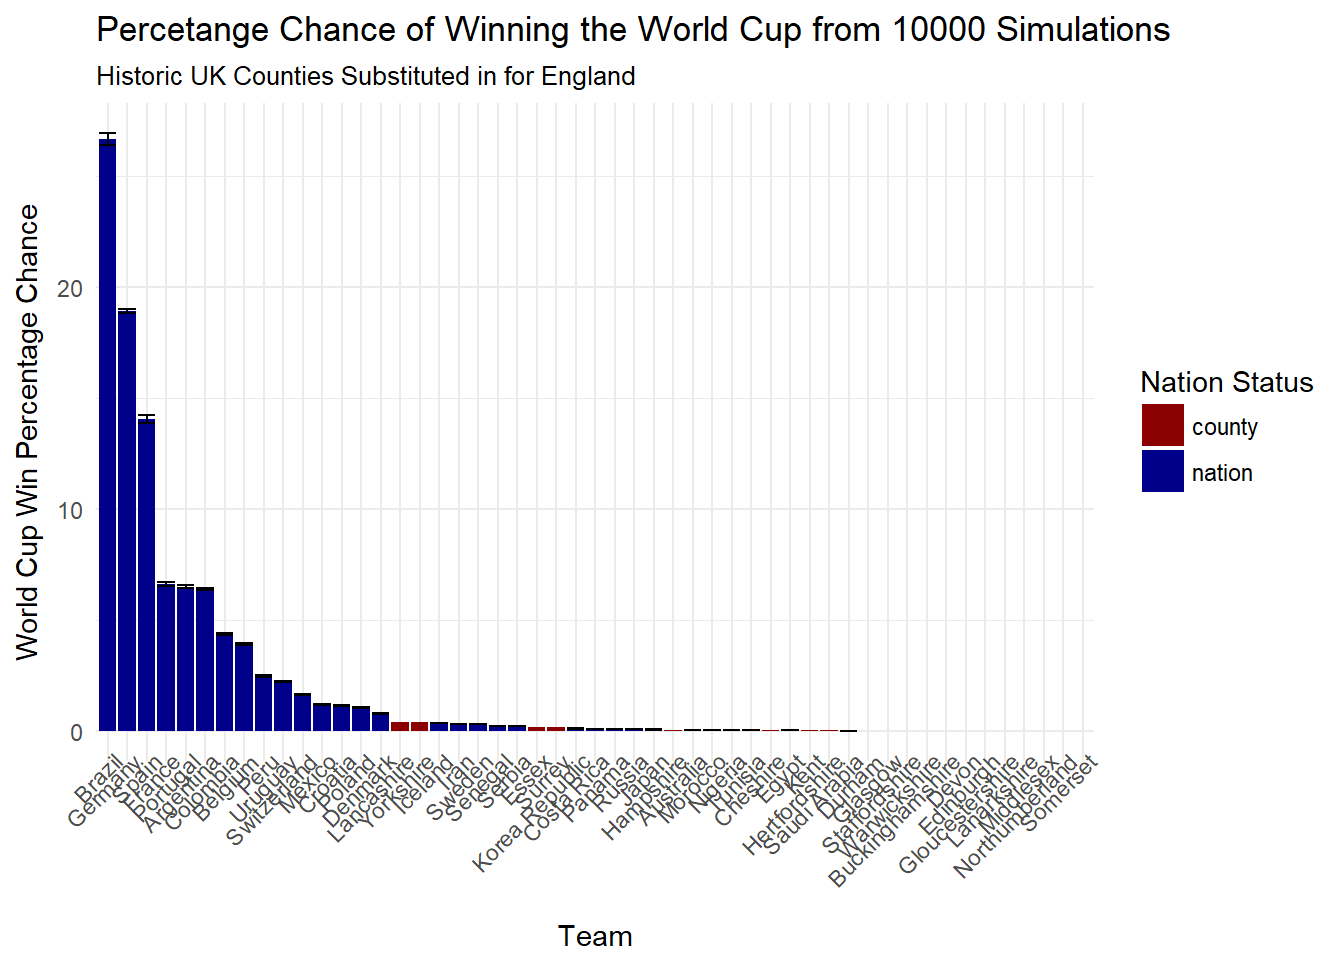
\includegraphics{2019-16-5-dixon-coles-1_files/figure-latex/plot_results-1.pdf}

As the colour gradient (from bottom right to top left) shows, the teams
we'd expect to do better are. Given the stochastic nature of football
though, there are some surprises. E.g. Blackburn only managing to draw
at home to Coventry.

A good sense of teams relative abilities can be seen in the league table
of results so far (assuming 3 points for a win, and 1 for a draw):

\begin{Shaded}
\begin{Highlighting}[]
\CommentTok{# function to melt results}
\CommentTok{# returns df with team and goals for and against for each match}
\NormalTok{melt_results <-}\StringTok{ }\ControlFlowTok{function}\NormalTok{(results_df) \{}
\NormalTok{  results_df }\OperatorTok
\StringTok{    }\CommentTok{# select only relevant columns}
\StringTok{    }\KeywordTok{select}\NormalTok{(home, away, hgoal, agoal) }\OperatorTok
\StringTok{    }\KeywordTok{gather}\NormalTok{(location, team,  }\OperatorTok{-}\NormalTok{hgoal, }\OperatorTok{-}\NormalTok{agoal) }\OperatorTok
\StringTok{    }\CommentTok{# calculate goals for/against the team}
\StringTok{    }\KeywordTok{mutate}\NormalTok{(}\DataTypeTok{g_for =} \KeywordTok{case_when}\NormalTok{(}
\NormalTok{      location }\OperatorTok{==}\StringTok{ "home"} \OperatorTok{~}\StringTok{ }\NormalTok{hgoal,}
\NormalTok{      location }\OperatorTok{==}\StringTok{ "away"} \OperatorTok{~}\StringTok{ }\NormalTok{agoal}
\NormalTok{    )) }\OperatorTok
\StringTok{    }\KeywordTok{mutate}\NormalTok{(}\DataTypeTok{g_ag =} \KeywordTok{case_when}\NormalTok{(}
\NormalTok{      location }\OperatorTok{==}\StringTok{ "home"} \OperatorTok{~}\StringTok{ }\NormalTok{agoal,}
\NormalTok{      location }\OperatorTok{==}\StringTok{ "away"} \OperatorTok{~}\StringTok{ }\NormalTok{hgoal}
\NormalTok{    )) }
\NormalTok{\}}

\CommentTok{# function to calculate points won and gd for each team}
\NormalTok{results_to_table <-}\StringTok{ }\ControlFlowTok{function}\NormalTok{(results_df) \{}
\NormalTok{  results_df }\OperatorTok
\StringTok{    }\CommentTok{# use above melting function}
\StringTok{    }\KeywordTok{melt_results}\NormalTok{(.) }\OperatorTok
\StringTok{    }\CommentTok{# 3 points for a win, 1 for a draw}
\StringTok{    }\KeywordTok{mutate}\NormalTok{(}\DataTypeTok{points =} \KeywordTok{case_when}\NormalTok{(}
\NormalTok{      g_for }\OperatorTok{>}\StringTok{ }\NormalTok{g_ag }\OperatorTok{~}\StringTok{ }\DecValTok{3}\NormalTok{,}
\NormalTok{      g_ag }\OperatorTok{>}\StringTok{ }\NormalTok{g_for }\OperatorTok{~}\StringTok{ }\DecValTok{0}\NormalTok{,}
\NormalTok{      g_for }\OperatorTok{==}\StringTok{ }\NormalTok{g_ag }\OperatorTok{~}\StringTok{ }\DecValTok{1}
\NormalTok{    )) }\OperatorTok
\StringTok{    }\CommentTok{# calculate goal difference for each match}
\StringTok{    }\KeywordTok{mutate}\NormalTok{(}\DataTypeTok{gd =}\NormalTok{ g_for }\OperatorTok{-}\StringTok{ }\NormalTok{g_ag) }\OperatorTok
\StringTok{    }\KeywordTok{group_by}\NormalTok{(team) }\OperatorTok
\StringTok{    }\CommentTok{# get the final statistics per team}
\StringTok{    }\KeywordTok{summarise}\NormalTok{(}\DataTypeTok{games_played =} \KeywordTok{n}\NormalTok{(),}
              \DataTypeTok{gf =} \KeywordTok{sum}\NormalTok{(g_for),}
              \DataTypeTok{ga =} \KeywordTok{sum}\NormalTok{(g_ag),}
              \DataTypeTok{gd =} \KeywordTok{sum}\NormalTok{(gd),}
              \DataTypeTok{points =} \KeywordTok{sum}\NormalTok{(points)) }\OperatorTok
\StringTok{    }\KeywordTok{arrange}\NormalTok{(}\OperatorTok{-}\NormalTok{points, }\OperatorTok{-}\NormalTok{gd, }\OperatorTok{-}\NormalTok{gf)}
\NormalTok{\}}

\CommentTok{# calculate league table for our played fixtures}
\NormalTok{league_table <-}\StringTok{ }\NormalTok{results  }\OperatorTok
\StringTok{  }\KeywordTok{filter}\NormalTok{(}\OperatorTok{!}\KeywordTok{is.na}\NormalTok{(hgoal)) }\OperatorTok
\StringTok{  }\KeywordTok{select}\NormalTok{(}\OperatorTok{-}\NormalTok{gameweek) }\OperatorTok
\StringTok{  }\KeywordTok{results_to_table}\NormalTok{(.) }\OperatorTok
\StringTok{  }\KeywordTok{print}\NormalTok{()}
\end{Highlighting}
\end{Shaded}

\begin{verbatim}
## # A tibble: 6 x 6
##   team             games_played    gf    ga    gd points
##   <chr>                   <int> <dbl> <dbl> <dbl>  <dbl>
## 1 Arsenal                     8    39     4    35     24
## 2 Blackburn_Rovers            8    23     6    17     19
## 3 Coventry_City               8    14     8     6     16
## 4 Dover_Athletic              8     8    15    -7      9
## 5 Enfield_Town                8     6    22   -16      3
## 6 Frimley_Green               8     2    37   -35      0
\end{verbatim}

Where teams positions are nicely rank ordered (the data for this example
is fairly curated so it's not that surprising).

\subsection{Predictions}\label{predictions}

With two rounds to go, there's still 6 fixtures we might want to predict
(to try and judge which team will end up where, or just to bet on the
remaining games).

This are:

\begin{Shaded}
\begin{Highlighting}[]
\CommentTok{# get the yet to be played matches}
\NormalTok{unplayed_games <-}\StringTok{ }\NormalTok{fixtures }\OperatorTok
\StringTok{  }\KeywordTok{filter}\NormalTok{(gameweek }\OperatorTok{>}\StringTok{ }\DecValTok{8}\NormalTok{) }\OperatorTok
\StringTok{  }\KeywordTok{print}\NormalTok{()}
\end{Highlighting}
\end{Shaded}

\begin{verbatim}
##               home             away gameweek
## 1    Coventry_City          Arsenal        9
## 2 Blackburn_Rovers   Dover_Athletic        9
## 3    Frimley_Green     Enfield_Town        9
## 4          Arsenal Blackburn_Rovers       10
## 5    Coventry_City    Frimley_Green       10
## 6   Dover_Athletic     Enfield_Town       10
\end{verbatim}

If we want to predict these results, we need to have data on the
strength of the teams above, but also, a good prior on what sort of
scores we should expect.

Using real data from the engsoccerdata package we can get the results of
all 48840 English football league games between August 1992 and May
2016. If we melt this to get the goals scored by each team by their
location we get a df of 97680 records of a teams performance in a game:

\begin{Shaded}
\begin{Highlighting}[]
\CommentTok{# load real data from the english league}
\NormalTok{real_data <-}\StringTok{ }\NormalTok{engsoccerdata}\OperatorTok{::}\NormalTok{england }\OperatorTok
\StringTok{  }\CommentTok{# filter out 'premier league era' matches}
\StringTok{  }\KeywordTok{filter}\NormalTok{(Season }\OperatorTok{>}\StringTok{ }\DecValTok{1991}\NormalTok{) }\OperatorTok
\StringTok{  }\CommentTok{# select only relevant columns}
\StringTok{  }\KeywordTok{select}\NormalTok{(home, }\DataTypeTok{away =}\NormalTok{ visitor, hgoal, }\DataTypeTok{agoal =}\NormalTok{ vgoal) }\OperatorTok
\StringTok{  }\CommentTok{# munge}
\StringTok{  }\KeywordTok{melt_results}\NormalTok{() }\OperatorTok
\StringTok{  }\KeywordTok{select}\NormalTok{(}\OperatorTok{-}\NormalTok{hgoal, }\OperatorTok{-}\NormalTok{agoal) }\OperatorTok
\StringTok{  }\KeywordTok{mutate}\NormalTok{(}\DataTypeTok{data =} \StringTok{"real"}\NormalTok{)}

\KeywordTok{head}\NormalTok{(real_data)}
\end{Highlighting}
\end{Shaded}

\begin{verbatim}
##   location    team g_for g_ag data
## 1     home Arsenal     0    1 real
## 2     home Arsenal     0    1 real
## 3     home Arsenal     2    1 real
## 4     home Arsenal     3    0 real
## 5     home Arsenal     3    0 real
## 6     home Arsenal     2    0 real
\end{verbatim}

Here every row shows a team that played a match (as it's sorted by
league then alphabetically, the first 6 records are all for Arsenal). It
also shows if the team played home or away. The data also shows the
goals scored by (e.g.) Arsenal in g\_for, and the goals they conceeded
in g\_ag.

If we plot the goals scored for each game, we get a nice humped
distribution with slightly offset peaks for home and away. That is to
say, in most games teams will score 0, 1, or 2 goals, and that scoring
more than 6 goals in a match is incredibly rare. The difference between
the home and away distributions mean that teams are slightly more likely
to score more if playing at home, compared to play away from home.

\begin{Shaded}
\begin{Highlighting}[]
\CommentTok{# plot goals scored home/away for real english football matches}
\NormalTok{p2 <-}\StringTok{ }\NormalTok{real_data }\OperatorTok
\StringTok{  }\KeywordTok{ggplot}\NormalTok{(., }\KeywordTok{aes}\NormalTok{(}\DataTypeTok{x =}\NormalTok{ g_for, }\DataTypeTok{fill =}\NormalTok{ location)) }\OperatorTok{+}
\StringTok{  }\CommentTok{# smooth densities}
\StringTok{  }\KeywordTok{geom_density}\NormalTok{(}\DataTypeTok{adjust =} \DecValTok{8}\NormalTok{, }\DataTypeTok{alpha =} \FloatTok{0.5}\NormalTok{) }\OperatorTok{+}
\StringTok{  }\KeywordTok{scale_fill_manual}\NormalTok{(}\DataTypeTok{values =} \KeywordTok{c}\NormalTok{(}\StringTok{"red"}\NormalTok{, }\StringTok{"blue"}\NormalTok{)) }\OperatorTok{+}
\StringTok{  }\KeywordTok{scale_x_continuous}\NormalTok{(}\DataTypeTok{breaks =} \DecValTok{0}\OperatorTok{:}\DecValTok{6}\NormalTok{) }\OperatorTok{+}
\StringTok{  }\KeywordTok{labs}\NormalTok{(}\DataTypeTok{title =} \StringTok{"Goals scored at home and away in English football"}\NormalTok{,}
       \DataTypeTok{subtitle =} \StringTok{"data from 48.8k matches 2000-2016"}\NormalTok{,}
       \DataTypeTok{x =} \StringTok{"goals scored"}\NormalTok{,}
       \DataTypeTok{y =} \StringTok{"density"}\NormalTok{) }\OperatorTok{+}
\StringTok{  }\KeywordTok{theme_minimal}\NormalTok{()}

\CommentTok{# plot}
\NormalTok{p2}
\end{Highlighting}
\end{Shaded}

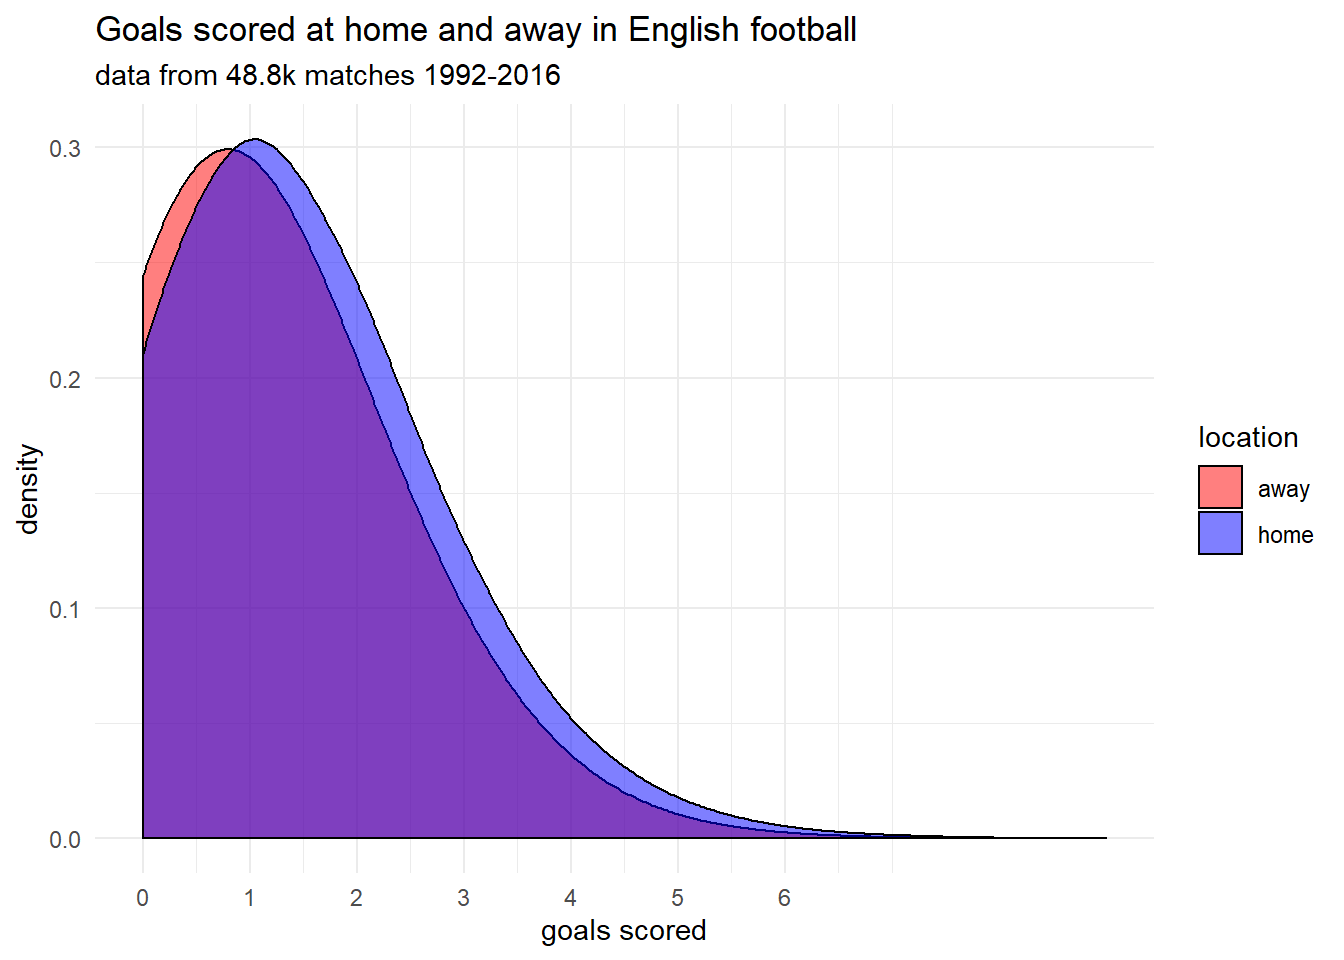
\includegraphics{2019-16-5-dixon-coles-1_files/figure-latex/plot_real_goal_distributions-1.pdf}

We can work out what the average difference between playing at home and
away is by taking the means of goals scored at home, and when playing
away:

\begin{Shaded}
\begin{Highlighting}[]
\CommentTok{# calculate mean home and away goals}
\NormalTok{real_data_means <-}\StringTok{ }\NormalTok{real_data }\OperatorTok
\StringTok{    }\KeywordTok{group_by}\NormalTok{(location) }\OperatorTok
\StringTok{    }\KeywordTok{summarise}\NormalTok{(}\DataTypeTok{mean_scored =} \KeywordTok{mean}\NormalTok{(g_for)) }\OperatorTok
\StringTok{  }\KeywordTok{print}\NormalTok{()}
\end{Highlighting}
\end{Shaded}

\begin{verbatim}
## # A tibble: 2 x 2
##   location mean_scored
##   <chr>          <dbl>
## 1 away            1.11
## 2 home            1.48
\end{verbatim}

Goals in games are both relatively sparse, and relatively stochastic,
football is a low scoring game where goals are evenly distributed
throughout the game. In theory any attack made by a team i has a
probability of being scored dependent upon the strength of team i's
attack (α\textsubscript{i}) which is independent of all the other
attacks that team has made.

(there is some reason to doubt this may be the case3, but for now this
is a fine generalisation)

By grouping all teams together into ``home'' and ``away'' categories (in
a league setting each team will play each other home and away so this
should average out) and taking the average number of goals scored per
match as the Poisson mean (λ) we can see how well our above graph fits a
simulated Poisson process.

\begin{Shaded}
\begin{Highlighting}[]
\CommentTok{# generate Poisson distributed vector with mean = real world mean}
\NormalTok{simulated_poisson <-}\StringTok{ }\NormalTok{real_data_means }\OperatorTok
\StringTok{  }\KeywordTok{split}\NormalTok{(}\DataTypeTok{f =}\NormalTok{ .}\OperatorTok{$}\NormalTok{location) }\OperatorTok
\StringTok{  }\KeywordTok{lapply}\NormalTok{(., }\ControlFlowTok{function}\NormalTok{(x) }\DataTypeTok{df =} \KeywordTok{data.frame}\NormalTok{(}\DataTypeTok{dist =} \KeywordTok{rpois}\NormalTok{(}\DecValTok{100000}\NormalTok{, x}\OperatorTok{$}\NormalTok{mean_scored),}
                                        \DataTypeTok{location =}\NormalTok{ x}\OperatorTok{$}\NormalTok{location)) }\OperatorTok
\StringTok{  }\CommentTok{# map it all together and label}
\StringTok{  }\KeywordTok{map_df}\NormalTok{(I) }\OperatorTok
\StringTok{  }\KeywordTok{mutate}\NormalTok{(}\DataTypeTok{data =} \StringTok{"simulated"}\NormalTok{) }

\CommentTok{# add these distributions to the plot}
\NormalTok{p2 }\OperatorTok{+}\StringTok{ }\KeywordTok{geom_density}\NormalTok{(}\DataTypeTok{data =}\NormalTok{ simulated_poisson, }\KeywordTok{aes}\NormalTok{(}\DataTypeTok{x =}\NormalTok{ dist), }\DataTypeTok{fill =} \OtherTok{NA}\NormalTok{, }\DataTypeTok{adjust =} \DecValTok{8}\NormalTok{, }\DataTypeTok{alpha =} \FloatTok{0.2}\NormalTok{) }\OperatorTok{+}
\StringTok{  }\KeywordTok{scale_fill_manual}\NormalTok{(}\DataTypeTok{values =} \KeywordTok{c}\NormalTok{(}\StringTok{"red"}\NormalTok{, }\StringTok{"blue"}\NormalTok{), }\DataTypeTok{guide =} \OtherTok{FALSE}\NormalTok{) }\OperatorTok{+}
\StringTok{  }\KeywordTok{facet_wrap}\NormalTok{(}\OperatorTok{~}\NormalTok{location)}
\end{Highlighting}
\end{Shaded}

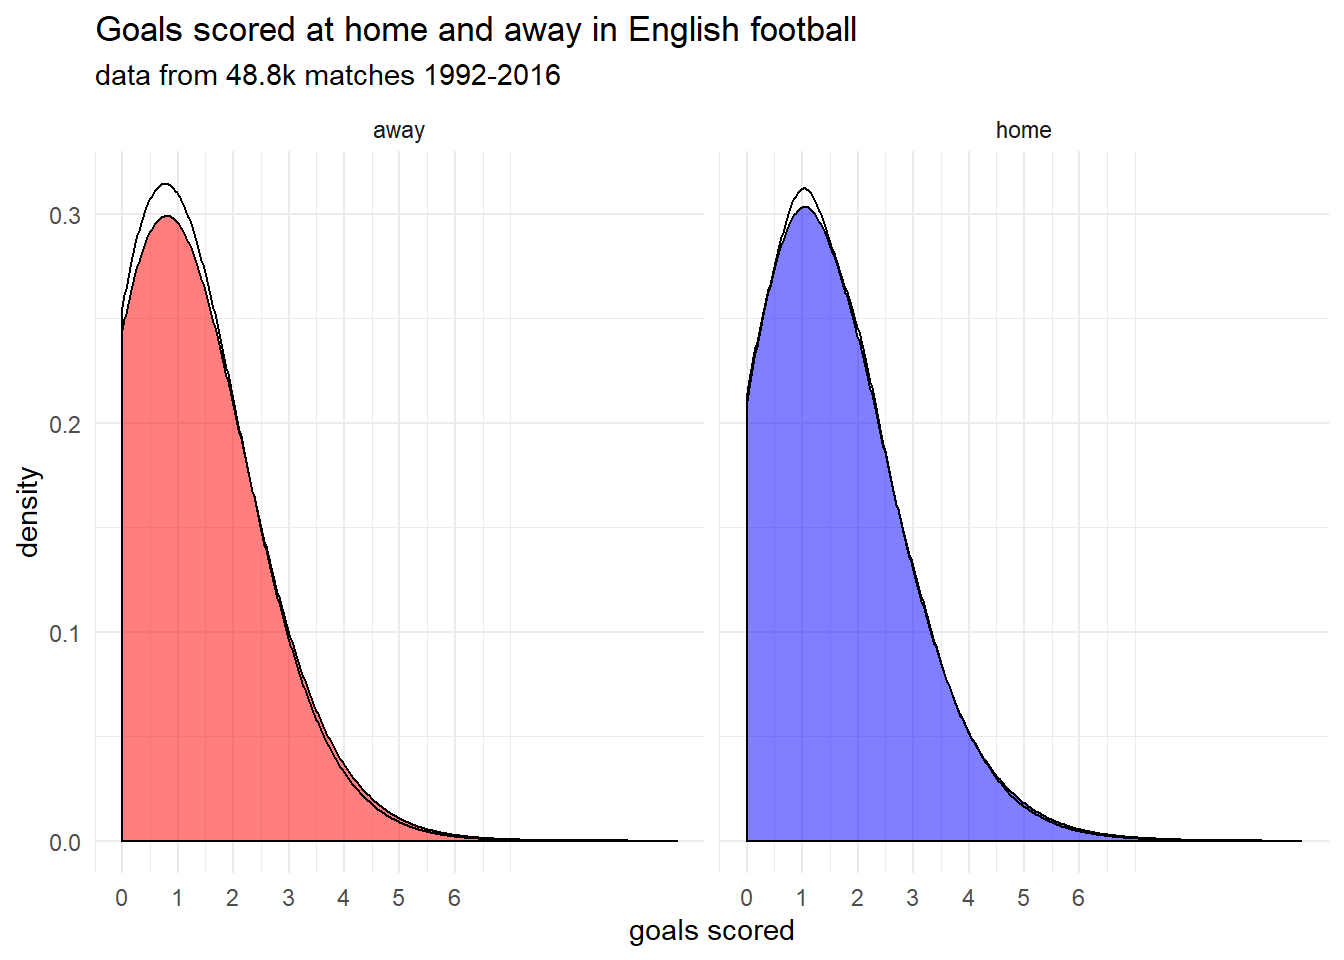
\includegraphics{2019-16-5-dixon-coles-1_files/figure-latex/simulated_poisson-1.pdf}

It's not perfect. But it's not a bad fit either. We can quantify how
well the Poisson distribution fits the data using a
\href{https://stats.stackexchange.com/questions/92627/how-to-use-the-chi-squared-test-to-determine-if-data-follow-the-poisson-distribu}{Chi
Squared test}.

\begin{Shaded}
\begin{Highlighting}[]
\CommentTok{# calc chi squared for home and away goals following Poisson distribution}
\NormalTok{calc_chi_squared <-}\StringTok{ }\ControlFlowTok{function}\NormalTok{(game_location) \{}
\NormalTok{  goals_scored <-}\StringTok{ }\KeywordTok{filter}\NormalTok{(real_data, location }\OperatorTok{==}\StringTok{ }\NormalTok{game_location)}\OperatorTok{$}\NormalTok{g_for}
  
\NormalTok{  observed_goal_counts <-}\StringTok{ }\KeywordTok{table}\NormalTok{(goals_scored)}

\NormalTok{  mean_goals <-}\StringTok{ }\KeywordTok{mean}\NormalTok{(goals_scored)}
  
\NormalTok{  probs =}\StringTok{ }\KeywordTok{dpois}\NormalTok{(}\KeywordTok{sort}\NormalTok{(}\KeywordTok{unique}\NormalTok{(goals_scored)), }\DataTypeTok{lambda =}\NormalTok{ mean_goals) }\OperatorTok
\StringTok{    }\KeywordTok{append}\NormalTok{(., }\DecValTok{1}\OperatorTok{-}\KeywordTok{sum}\NormalTok{(.))}
  
  \CommentTok{# the chi squared test}
\NormalTok{  test <-}\StringTok{ }\KeywordTok{chisq.test}\NormalTok{(}\DataTypeTok{x =} \KeywordTok{c}\NormalTok{(observed_goal_counts,}\DecValTok{0}\NormalTok{), }\DataTypeTok{p =}\NormalTok{ probs, }\DataTypeTok{simulate.p.value =} \OtherTok{TRUE}\NormalTok{)}
\NormalTok{  test}\OperatorTok{$}\NormalTok{data.name <-}\StringTok{ }\NormalTok{game_location}
  
  \KeywordTok{return}\NormalTok{(test)}
\NormalTok{\}}

\CommentTok{# run test for both home and away goals}
\KeywordTok{lapply}\NormalTok{(}\KeywordTok{c}\NormalTok{(}\StringTok{"home"}\NormalTok{, }\StringTok{"away"}\NormalTok{), calc_chi_squared)}
\end{Highlighting}
\end{Shaded}

\begin{verbatim}
## [[1]]
## 
##  Chi-squared test for given probabilities with simulated p-value
##  (based on 2000 replicates)
## 
## data:  home
## X-squared = 53.752, df = NA, p-value = 0.001499
## 
## 
## [[2]]
## 
##  Chi-squared test for given probabilities with simulated p-value
##  (based on 2000 replicates)
## 
## data:  away
## X-squared = 38.599, df = NA, p-value = 0.01599
\end{verbatim}

It's actually perhaps not as significant as might be expected given the
sheer amount of observations we have (see above reservations about
modelling goals as a Poisson process) but it's clearly not the worst
approximation either. The p-values \textless{} 0.05 for both home and
away match data show we have a good reason to reject the null hypothesis
that the data is not a Poisson distribution.

If we think that goals scored represents some Poisson process, it can be
modelled using the equation which underlies the Pisson distribution. For
a given interval (one match), the probability of x events (goals scored)
in that interval will be:

\(P(x) = \frac{\lambda^{x}e^{-\lambda}}{x!}\)

The simplest model we can produce is to estimate λ as each team's attack
rating (henceforth α\textsubscript{i}) which is equal to observed mean
rate of goals for that team.

That is the say the probability of team i scoring x goals against team j
is:

\(P(X_{i,j} = x) = \frac{\alpha_{i}^{x}e^{-\alpha_{i}}}{x!}\)

where α\textsubscript{i} is the sum of all goals scored divided by the
total number of matches:

\(\alpha_{i} = \frac{1}{N}\sum_{n=1}^{N} x\)

grouping by teams makes this easy to calculate:

\begin{Shaded}
\begin{Highlighting}[]
\NormalTok{basic_model <-}\StringTok{ }\NormalTok{results }\OperatorTok
\StringTok{  }\KeywordTok{melt_results}\NormalTok{() }\OperatorTok
\StringTok{  }\KeywordTok{group_by}\NormalTok{(team) }\OperatorTok
\StringTok{  }\CommentTok{# we'll use the goals scored to model the attack}
\StringTok{  }\CommentTok{# and goals conceeded to measure defence rating}
\StringTok{  }\KeywordTok{summarise}\NormalTok{(}\DataTypeTok{alpha =} \KeywordTok{mean}\NormalTok{(g_for),}
            \DataTypeTok{beta =} \KeywordTok{mean}\NormalTok{(g_ag)) }\OperatorTok
\StringTok{  }\KeywordTok{print}\NormalTok{()}
\end{Highlighting}
\end{Shaded}

\begin{verbatim}
## # A tibble: 6 x 3
##   team             alpha  beta
##   <chr>            <dbl> <dbl>
## 1 Arsenal           4.88  0.5 
## 2 Blackburn_Rovers  2.88  0.75
## 3 Coventry_City     1.75  1   
## 4 Dover_Athletic    1     1.88
## 5 Enfield_Town      0.75  2.75
## 6 Frimley_Green     0.25  4.62
\end{verbatim}

(we'll come on to the beta parameter in a bit- where alpha is the
average scoring rate, beta is the average condeeding rate).

If we take Coventry's remaining two games as examples we can see that
they are yet to play Arsenal and Frimley Green at home

\begin{Shaded}
\begin{Highlighting}[]
\NormalTok{coventry_games <-}\StringTok{ }\NormalTok{unplayed_games }\OperatorTok
\StringTok{  }\CommentTok{# filter out Coventry City's remaining fixtures}
\StringTok{  }\KeywordTok{filter}\NormalTok{(}\KeywordTok{grepl}\NormalTok{(}\StringTok{"Coventry_City"}\NormalTok{, home)) }\OperatorTok
\StringTok{  }\KeywordTok{print}\NormalTok{()}
\end{Highlighting}
\end{Shaded}

\begin{verbatim}
##            home          away gameweek
## 1 Coventry_City       Arsenal        9
## 2 Coventry_City Frimley_Green       10
\end{verbatim}

And we can take the attack rating (α) of each team and use it to
estimate the results

\begin{Shaded}
\begin{Highlighting}[]
\CommentTok{# get the attack ratings of all teams}
\NormalTok{team_alphas <-}\StringTok{ }\NormalTok{basic_model}\OperatorTok{$}\NormalTok{alpha }\OperatorTok\StringTok{ `}\DataTypeTok{names<-}\StringTok{`}\NormalTok{(basic_model}\OperatorTok{$}\NormalTok{team)}

\CommentTok{# assume goals scored for each team will be it's attack rating}
\NormalTok{e_results <-}\StringTok{ }\KeywordTok{paste}\NormalTok{(team_alphas[coventry_games}\OperatorTok{$}\NormalTok{home],}
\NormalTok{                   team_alphas[coventry_games}\OperatorTok{$}\NormalTok{away],}
                   \DataTypeTok{sep =} \StringTok{"-"}\NormalTok{) }\OperatorTok
\StringTok{  }\CommentTok{# name each match with the teams competing}
\StringTok{  `}\DataTypeTok{names<-}\StringTok{`}\NormalTok{(}\KeywordTok{c}\NormalTok{(}\KeywordTok{paste}\NormalTok{(coventry_games}\OperatorTok{$}\NormalTok{home, coventry_games}\OperatorTok{$}\NormalTok{away, }\DataTypeTok{sep =} \StringTok{"-"}\NormalTok{))) }\OperatorTok
\StringTok{  }\KeywordTok{print}\NormalTok{()}
\end{Highlighting}
\end{Shaded}

\begin{verbatim}
##       Coventry_City-Arsenal Coventry_City-Frimley_Green 
##                "1.75-4.875"                 "1.75-0.25"
\end{verbatim}

These aren't ridiculous estimates by any stretch but it's clear
something is up. It's pretty intuitive that Coventry City would be
expected to score more goals at home to Frimley Green than at home to
Arsenal.

We can account for this by introducing an opposing team defence paramter
β\textsubscript{j}. In our very simple model this will be estimating by
taking the average rate a team conceedes goals. As with the attack
rating, this is the calculated as the sum of all goals conceeded divided
by number of matches. We'll then multiply α\textsubscript{i} and
β\textsubscript{j} together to get the score estimate:

\begin{Shaded}
\begin{Highlighting}[]
\CommentTok{# get and name the defence rating for each team}
\NormalTok{team_betas <-}\StringTok{ }\NormalTok{basic_model}\OperatorTok{$}\NormalTok{beta }\OperatorTok\StringTok{ `}\DataTypeTok{names<-}\StringTok{`}\NormalTok{(basic_model}\OperatorTok{$}\NormalTok{team)}

\CommentTok{# assume the goals scored will be the attack rating of the team times }
\CommentTok{# the defence rating of it's opponent}
\NormalTok{e_results <-}\StringTok{ }\KeywordTok{paste}\NormalTok{(}\KeywordTok{round}\NormalTok{(team_alphas[coventry_games}\OperatorTok{$}\NormalTok{home]}\OperatorTok{*}
\StringTok{                           }\NormalTok{team_betas[coventry_games}\OperatorTok{$}\NormalTok{away], }\DecValTok{3}\NormalTok{),}
                   \KeywordTok{round}\NormalTok{(team_alphas[coventry_games}\OperatorTok{$}\NormalTok{away]}\OperatorTok{*}
\StringTok{                           }\NormalTok{team_betas[coventry_games}\OperatorTok{$}\NormalTok{home], }\DecValTok{3}\NormalTok{),}
                   \DataTypeTok{sep =} \StringTok{"-"}\NormalTok{) }\OperatorTok
\StringTok{  `}\DataTypeTok{names<-}\StringTok{`}\NormalTok{(}\KeywordTok{c}\NormalTok{(}\KeywordTok{paste}\NormalTok{(coventry_games}\OperatorTok{$}\NormalTok{home, coventry_games}\OperatorTok{$}\NormalTok{away, }\DataTypeTok{sep =} \StringTok{"-"}\NormalTok{))) }\OperatorTok
\StringTok{  }\KeywordTok{print}\NormalTok{()}
\end{Highlighting}
\end{Shaded}

\begin{verbatim}
##       Coventry_City-Arsenal Coventry_City-Frimley_Green 
##               "0.875-4.875"                "8.094-0.25"
\end{verbatim}

The opposition scores remain the same because Coventry have on average
conceeded 1 goal per game.

Coventry's predicted goals though has diverged with them now predicted
to score less than a goal against Arsenal and to score 8(!) against
Frimley Green, both of which sound reasonable (when you consider that
Frimley Green are a team of amateurs).

However, we're also missing one final piece of the model we'll finish
with today. Recall modelling the English football data from 1992
onwards, we were left with a difference between the home scoring rate
and the away scoring rate.

\begin{Shaded}
\begin{Highlighting}[]
\CommentTok{# reprint what we calculated earlier}
\NormalTok{real_data_means}
\end{Highlighting}
\end{Shaded}

\begin{verbatim}
## # A tibble: 2 x 2
##   location mean_scored
##   <chr>          <dbl>
## 1 away            1.11
## 2 home            1.48
\end{verbatim}

It's pretty common knowledge that football teams do better at home, so
we'll want to factor that in. A simple estimate is to divide the mean
home goals/game by the mean away goals/game.

We'll call this parameter γ and can be formalised as the sum of home
goals (which we'll refer to as X from now on) divided by the sum of away
goals (Y)

\(\gamma = \frac{\sum{X}}{\sum{Y}}\)

\begin{Shaded}
\begin{Highlighting}[]
\CommentTok{# the home advantage is how much easier it is to score at home}
\NormalTok{home_advantage_gamma <-}\StringTok{ }\KeywordTok{sum}\NormalTok{(results}\OperatorTok{$}\NormalTok{hgoal) }\OperatorTok{/}\StringTok{ }\KeywordTok{sum}\NormalTok{(results}\OperatorTok{$}\NormalTok{agoal)}

\NormalTok{e_results <-}\StringTok{ }\KeywordTok{paste}\NormalTok{(}\KeywordTok{round}\NormalTok{(team_alphas[coventry_games}\OperatorTok{$}\NormalTok{home]}\OperatorTok{*}
\StringTok{                           }\NormalTok{team_betas[coventry_games}\OperatorTok{$}\NormalTok{away] }\OperatorTok{*}\StringTok{ }
\StringTok{                           }\CommentTok{# add in home advantage for home team}
\StringTok{                           }\NormalTok{home_advantage_gamma, }\DecValTok{3}\NormalTok{),}
                   \KeywordTok{round}\NormalTok{(team_alphas[coventry_games}\OperatorTok{$}\NormalTok{away]}\OperatorTok{*}
\StringTok{                           }\NormalTok{team_betas[coventry_games}\OperatorTok{$}\NormalTok{home], }\DecValTok{3}\NormalTok{),}
                   \DataTypeTok{sep =} \StringTok{"-"}\NormalTok{) }\OperatorTok
\StringTok{  `}\DataTypeTok{names<-}\StringTok{`}\NormalTok{(}\KeywordTok{c}\NormalTok{(}\KeywordTok{paste}\NormalTok{(coventry_games}\OperatorTok{$}\NormalTok{home, coventry_games}\OperatorTok{$}\NormalTok{away, }\DataTypeTok{sep =} \StringTok{"-"}\NormalTok{))) }\OperatorTok
\StringTok{  }\KeywordTok{print}\NormalTok{()}
\end{Highlighting}
\end{Shaded}

\begin{verbatim}
##       Coventry_City-Arsenal Coventry_City-Frimley_Green 
##               "0.955-4.875"                 "8.83-0.25"
\end{verbatim}

Which tilts the scales a little towards Coventry's favour but (as we'd
expect- home advantage can only go so far) doesn't affect the results
too much.

Now we have a method to predict matches, we can use this on the
remaining 6 nice and easily:

\begin{Shaded}
\begin{Highlighting}[]
\CommentTok{# simplify to just gamma}
\NormalTok{gamma <-}\StringTok{ }\NormalTok{home_advantage_gamma}

\CommentTok{# wrap the above into a function for home and away teams}
\NormalTok{predict_results <-}\StringTok{ }\ControlFlowTok{function}\NormalTok{(home, away, parameters) \{}
\NormalTok{  e_goals_home <-}\StringTok{ }\NormalTok{parameters}\OperatorTok{$}\NormalTok{alpha[home]}\OperatorTok{*}\NormalTok{parameters}\OperatorTok{$}\NormalTok{beta[away] }\OperatorTok{*}\StringTok{ }\NormalTok{gamma}
\NormalTok{  e_goals_away <-}\StringTok{ }\NormalTok{parameters}\OperatorTok{$}\NormalTok{alpha[away]}\OperatorTok{*}\NormalTok{parameters}\OperatorTok{$}\NormalTok{beta[home]}
  
  \CommentTok{# output a df of expected goals for home and away teams}
\NormalTok{  df <-}\StringTok{ }\KeywordTok{data.frame}\NormalTok{(}\DataTypeTok{home =}\NormalTok{ home, }\DataTypeTok{away =}\NormalTok{ away,}
                   \DataTypeTok{e_hgoal =}\NormalTok{ e_goals_home, }\DataTypeTok{e_agoal =}\NormalTok{ e_goals_away)}
  \KeywordTok{return}\NormalTok{(df)}
\NormalTok{\}}

\CommentTok{# convert the basic_model df into a list with $attack and $defence parameters}
\CommentTok{# for each team}
\NormalTok{basic_parameters <-}\StringTok{ }\NormalTok{basic_model }\OperatorTok
\StringTok{  }\CommentTok{# rename scored/conceeded to attack/defence}
\StringTok{  }\KeywordTok{select}\NormalTok{(}\OperatorTok{-}\NormalTok{team) }\OperatorTok
\StringTok{  }\CommentTok{# convert to a list and name each element}
\StringTok{  }\KeywordTok{as.list}\NormalTok{() }\OperatorTok
\StringTok{  }\KeywordTok{lapply}\NormalTok{(., }\ControlFlowTok{function}\NormalTok{(x)\{}\KeywordTok{names}\NormalTok{(x) <-}\StringTok{ }\NormalTok{teams;}\KeywordTok{return}\NormalTok{(x)\})}

\CommentTok{# predict results using the function defined above and the list of parameters}
\CommentTok{# could use e.g. mapply here but I prefer the map2 grammar}
\CommentTok{# run the predict results function over each game consisting of $home and $away}
\NormalTok{predicted_fixtures <-}\StringTok{ }\KeywordTok{map2_df}\NormalTok{(unplayed_games}\OperatorTok{$}\NormalTok{home, unplayed_games}\OperatorTok{$}\NormalTok{away, }
\NormalTok{                    predict_results,}
                    \CommentTok{# parameters forms an extra argument that does not vary}
\NormalTok{                    basic_parameters) }\OperatorTok
\StringTok{  }\CommentTok{# round the outputs}
\StringTok{  }\KeywordTok{mutate_if}\NormalTok{(is.numeric, round, }\DataTypeTok{digits =} \DecValTok{2}\NormalTok{) }\OperatorTok
\StringTok{  }\KeywordTok{print}\NormalTok{()}
\end{Highlighting}
\end{Shaded}

\begin{verbatim}
##               home             away e_hgoal e_agoal
## 1    Coventry_City          Arsenal    0.95    4.88
## 2 Blackburn_Rovers   Dover_Athletic    5.88    0.75
## 3    Frimley_Green     Enfield_Town    0.75    3.47
## 4          Arsenal Blackburn_Rovers    3.99    1.44
## 5    Coventry_City    Frimley_Green    8.83    0.25
## 6   Dover_Athletic     Enfield_Town    3.00    1.41
\end{verbatim}

All of which look reasonable, if maybe a little bullish on the `better'
teams prospects.

However, while this is good for back of the envelope predictions, we
know that this is a very basic model. If we want to improve it, first we
must quantify how good it is.

In order to do this we can use the results we have from the first 8
weeks of matches as training data. We know what the `correct' scores are
for these matches, so if our model is good, it will predict similar
scores to those observed.

Remember that for the Poisson distribution, the probability of x goals
in one match is

\(P(x) = \frac{\lambda^{x}e^{-\lambda}}{x!}\)

The expected value of the Poisson distribution is equal to λ, so we can
plug λ as our predicted goals, and x as the actual goals, and calculate
the probability of that results occuring \emph{given} the
attack/defence/home advantage parameters that we think are correct.

We then do this for all the matches played and get the likelihood for
the home and away teams scores given the model:

\begin{Shaded}
\begin{Highlighting}[]
\CommentTok{# 'predict' the already played matches using our function}
\NormalTok{predicted_results <-}\StringTok{ }\KeywordTok{map2_df}\NormalTok{(results}\OperatorTok{$}\NormalTok{home, results}\OperatorTok{$}\NormalTok{away, }
\NormalTok{                    predict_results,}
\NormalTok{                    basic_parameters) }\OperatorTok
\StringTok{  }\KeywordTok{mutate_if}\NormalTok{(is.numeric, round, }\DataTypeTok{digits =} \DecValTok{2}\NormalTok{) }\OperatorTok
\StringTok{  }\KeywordTok{print}\NormalTok{()}
\end{Highlighting}
\end{Shaded}

\begin{verbatim}
##                home             away e_hgoal e_agoal
## 1    Dover_Athletic    Coventry_City    1.09    3.28
## 2      Enfield_Town Blackburn_Rovers    0.61    7.91
## 3     Frimley_Green          Arsenal    0.14   22.55
## 4           Arsenal     Enfield_Town   14.62    0.38
## 5  Blackburn_Rovers    Coventry_City    3.14    1.31
## 6     Frimley_Green   Dover_Athletic    0.51    4.62
## 7  Blackburn_Rovers    Frimley_Green   14.51    0.19
## 8     Coventry_City     Enfield_Town    5.25    0.75
## 9    Dover_Athletic          Arsenal    0.55    9.14
## 10          Arsenal    Coventry_City    5.32    0.88
## 11   Dover_Athletic Blackburn_Rovers    0.82    5.39
## 12     Enfield_Town    Frimley_Green    3.78    0.69
## 13 Blackburn_Rovers          Arsenal    1.57    3.66
## 14     Enfield_Town   Dover_Athletic    1.53    2.75
## 15    Frimley_Green    Coventry_City    0.27    8.09
## 16          Arsenal    Frimley_Green   24.60    0.12
## 17 Blackburn_Rovers     Enfield_Town    8.62    0.56
## 18    Coventry_City   Dover_Athletic    3.58    1.00
## 19    Coventry_City Blackburn_Rovers    1.43    2.88
## 20   Dover_Athletic    Frimley_Green    5.05    0.47
## 21     Enfield_Town          Arsenal    0.41   13.41
## 22          Arsenal   Dover_Athletic    9.97    0.50
## 23     Enfield_Town    Coventry_City    0.82    4.81
## 24    Frimley_Green Blackburn_Rovers    0.20   13.30
\end{verbatim}

\begin{Shaded}
\begin{Highlighting}[]
\CommentTok{# calculate the likelihood of each home/away team actually scoring that many goals}
\CommentTok{# given the parameters for attack/defence supplied}
\NormalTok{likelihoods <-}\StringTok{ }\KeywordTok{data.frame}\NormalTok{(}\DataTypeTok{lik_hgoal =} \KeywordTok{dpois}\NormalTok{(results}\OperatorTok{$}\NormalTok{hgoal,}
\NormalTok{                                            predicted_results}\OperatorTok{$}\NormalTok{e_hgoal),}
                          \DataTypeTok{lik_agoal =} \KeywordTok{dpois}\NormalTok{(results}\OperatorTok{$}\NormalTok{agoal,}
\NormalTok{                                            predicted_results}\OperatorTok{$}\NormalTok{e_agoal)) }\OperatorTok
\StringTok{  }\CommentTok{# round the probabilities}
\StringTok{  }\KeywordTok{mutate_all}\NormalTok{(round, }\DecValTok{4}\NormalTok{) }\OperatorTok
\StringTok{  }\CommentTok{# bind likelihoods to results}
\StringTok{  }\KeywordTok{cbind}\NormalTok{(results, . ) }\OperatorTok
\StringTok{  }\CommentTok{# bind in predictions}
\StringTok{  }\KeywordTok{left_join}\NormalTok{(., predicted_results, }\DataTypeTok{by =} \KeywordTok{c}\NormalTok{(}\StringTok{"home"}\NormalTok{, }\StringTok{"away"}\NormalTok{)) }\OperatorTok
\StringTok{  }\CommentTok{# select useful parameters}
\StringTok{  }\KeywordTok{select}\NormalTok{(home, away, hgoal, e_hgoal, lik_hgoal, agoal, e_agoal, lik_agoal) }\OperatorTok
\StringTok{  }\KeywordTok{print}\NormalTok{()}
\end{Highlighting}
\end{Shaded}

\begin{verbatim}
##                home             away hgoal e_hgoal lik_hgoal agoal e_agoal
## 1    Dover_Athletic    Coventry_City     0    1.09    0.3362     3    3.28
## 2      Enfield_Town Blackburn_Rovers     0    0.61    0.5434     3    7.91
## 3     Frimley_Green          Arsenal     0    0.14    0.8694     8   22.55
## 4           Arsenal     Enfield_Town     5   14.62    0.0025     0    0.38
## 5  Blackburn_Rovers    Coventry_City     1    3.14    0.1359     1    1.31
## 6     Frimley_Green   Dover_Athletic     1    0.51    0.3063     2    4.62
## 7  Blackburn_Rovers    Frimley_Green     6   14.51    0.0065     0    0.19
## 8     Coventry_City     Enfield_Town     2    5.25    0.0723     1    0.75
## 9    Dover_Athletic          Arsenal     1    0.55    0.3173     3    9.14
## 10          Arsenal    Coventry_City     3    5.32    0.1228     1    0.88
## 11   Dover_Athletic Blackburn_Rovers     1    0.82    0.3612     2    5.39
## 12     Enfield_Town    Frimley_Green     1    3.78    0.0863     0    0.69
## 13 Blackburn_Rovers          Arsenal     0    1.57    0.2080     2    3.66
## 14     Enfield_Town   Dover_Athletic     1    1.53    0.3313     2    2.75
## 15    Frimley_Green    Coventry_City     0    0.27    0.7634     3    8.09
## 16          Arsenal    Frimley_Green    10   24.60    0.0005     0    0.12
## 17 Blackburn_Rovers     Enfield_Town     4    8.62    0.0415     0    0.56
## 18    Coventry_City   Dover_Athletic     1    3.58    0.0998     0    1.00
## 19    Coventry_City Blackburn_Rovers     1    1.43    0.3422     2    2.88
## 20   Dover_Athletic    Frimley_Green     2    5.05    0.0817     0    0.47
## 21     Enfield_Town          Arsenal     2    0.41    0.0558     4   13.41
## 22          Arsenal   Dover_Athletic     4    9.97    0.0193     0    0.50
## 23     Enfield_Town    Coventry_City     1    0.82    0.3612     2    4.81
## 24    Frimley_Green Blackburn_Rovers     1    0.20    0.1637     5   13.30
##    lik_agoal
## 1     0.2213
## 2     0.0303
## 3     0.0003
## 4     0.6839
## 5     0.3535
## 6     0.1052
## 7     0.8270
## 8     0.3543
## 9     0.0137
## 10    0.3650
## 11    0.0663
## 12    0.5016
## 13    0.1724
## 14    0.2417
## 15    0.0271
## 16    0.8869
## 17    0.5712
## 18    0.3679
## 19    0.2328
## 20    0.6250
## 21    0.0020
## 22    0.6065
## 23    0.0943
## 24    0.0058
\end{verbatim}

If we sum the log of those likelihood values we get a measure of how
wrong overall our predictions are:

\begin{Shaded}
\begin{Highlighting}[]
\NormalTok{log_likehood <-}\StringTok{ }\KeywordTok{sum}\NormalTok{(}\KeywordTok{log}\NormalTok{(likelihoods}\OperatorTok{$}\NormalTok{lik_hgoal), }\KeywordTok{log}\NormalTok{(likelihoods}\OperatorTok{$}\NormalTok{lik_agoal)) }\OperatorTok{*}\StringTok{ }\OperatorTok{-}\DecValTok{1}

\NormalTok{log_likehood}
\end{Highlighting}
\end{Shaded}

\begin{verbatim}
## [1] 105.995
\end{verbatim}

(n.b. there'll be some rounding errors- especially on the pre-log
probabilities, but this will suffice for now)

To get an idea of whether or not this is good, let's quickly run the
model with all the parameters set to zero. Given that we're pretty sure
that at least Arsenal will be a lot better than Frimley Green, this
model should do worse than our basic model above.

If it indeed does fit the results worse we will get a greater error
term- the log likelihood sum

\begin{Shaded}
\begin{Highlighting}[]
\CommentTok{# do the same but set each teams attack and defence to 1}
\CommentTok{# expect model to be worse as assumes all teams are equal}
\NormalTok{equal_parameters <-}\StringTok{ }\KeywordTok{list}\NormalTok{(}
  \DataTypeTok{alpha =} \KeywordTok{rep}\NormalTok{(}\DecValTok{1}\NormalTok{, }\KeywordTok{length}\NormalTok{(teams)) }\OperatorTok\StringTok{ `}\DataTypeTok{names<-}\StringTok{`}\NormalTok{(teams),}
  \DataTypeTok{beta =} \KeywordTok{rep}\NormalTok{(}\DecValTok{1}\NormalTok{, }\KeywordTok{length}\NormalTok{(teams)) }\OperatorTok\StringTok{ `}\DataTypeTok{names<-}\StringTok{`}\NormalTok{(teams)}
\NormalTok{)}

\CommentTok{# predict results and munge through to find sum of log likelihoods}
\NormalTok{worse_log_likelihood <-}\StringTok{ }\KeywordTok{map2_df}\NormalTok{(results}\OperatorTok{$}\NormalTok{home, results}\OperatorTok{$}\NormalTok{away, }
\NormalTok{                    predict_results,}
\NormalTok{                    equal_parameters) }\OperatorTok
\StringTok{  }\KeywordTok{mutate_if}\NormalTok{(is.numeric, round, }\DataTypeTok{digits =} \DecValTok{2}\NormalTok{) }\OperatorTok
\StringTok{  }\CommentTok{# take the log probability straight away this time}
\StringTok{  }\KeywordTok{mutate}\NormalTok{(}\DataTypeTok{lik_hgoal =} \KeywordTok{dpois}\NormalTok{(results}\OperatorTok{$}\NormalTok{hgoal, e_hgoal, }\DataTypeTok{log =} \OtherTok{TRUE}\NormalTok{),}
         \DataTypeTok{lik_agoal =} \KeywordTok{dpois}\NormalTok{(results}\OperatorTok{$}\NormalTok{agoal, e_agoal, }\DataTypeTok{log =} \OtherTok{TRUE}\NormalTok{)) }\OperatorTok
\StringTok{  }\KeywordTok{select}\NormalTok{(lik_hgoal, lik_agoal) }\OperatorTok
\StringTok{  }\KeywordTok{map_dbl}\NormalTok{(sum) }\OperatorTok
\StringTok{  }\KeywordTok{sum}\NormalTok{(.) }\OperatorTok{*}\StringTok{ }\OperatorTok{-}\DecValTok{1} 

\NormalTok{worse_log_likelihood}
\end{Highlighting}
\end{Shaded}

\begin{verbatim}
## [1] 112.618
\end{verbatim}

The worse log likelihood (112.6) is worse (only a bit though) than the
106.0 we previously. This suggests that either the teams are actually
quite equal, or that our basic model wasn't all that good.

\subsection{Parameter Optimisation}\label{parameter-optimisation}

There will exist some parameters (α and β for each team, and γ for the
home field advantage) that will minimise this negative log likehood.
That is to say, they will predict the results of the already played
games most accurately.

If we want to find those we can use the optim() function in the stats
package. This will take a vector of paramaters and iterate while
slightly changing their values until it gets the lowest value it can
find as the output for a supplied function. It also takes a df of
results between teams. The results of these games are predicted and then
checked against this actually observed data.

At the end, I've also set the function to pass some information from
each iteration into the global environment, namely, the iteration number
(i), the parameter values the optim() function has chosen for this
iteration, and the negative log likelihood of those parameters- the
likelihood of the observed scores if those parameters are correct.

\begin{Shaded}
\begin{Highlighting}[]
\NormalTok{optimise_params <-}\StringTok{ }\ControlFlowTok{function}\NormalTok{(parameters, results) \{}
  \CommentTok{# form the parameters back into a list}
  \CommentTok{# parameters names alpha (attack), beta (defense), and gamma (hfa)}
\NormalTok{  param_list <-}\StringTok{ }\KeywordTok{relist_params}\NormalTok{(parameters)}
  
  \CommentTok{# predict the expected results for the games that have been played}
\NormalTok{  e_results <-}\StringTok{ }\KeywordTok{map2_df}\NormalTok{(results}\OperatorTok{$}\NormalTok{home, results}\OperatorTok{$}\NormalTok{away, }
\NormalTok{                      predict_results,}
\NormalTok{                      param_list)}
  
  \CommentTok{# calculate the negative log likelihood of those predictions}
  \CommentTok{# given the parameters how likely are those scores}
\NormalTok{  neg_log_likelihood <-}\StringTok{ }\KeywordTok{calculate_log_likelihood}\NormalTok{(results, e_results)}
  
  \CommentTok{# capture the parameters and likelihood at each loop}
  \CommentTok{# only do it if i is initialised}
  \ControlFlowTok{if}\NormalTok{(}\KeywordTok{exists}\NormalTok{(}\StringTok{"i"}\NormalTok{)) \{}
\NormalTok{    i <<-}\StringTok{ }\NormalTok{i }\OperatorTok{+}\StringTok{ }\DecValTok{1}
\NormalTok{    current_parameters[[i]] <<-}\StringTok{ }\NormalTok{parameters}
\NormalTok{    current_nll[[i]] <<-}\StringTok{ }\NormalTok{neg_log_likelihood}
\NormalTok{  \}}
  
  \CommentTok{# return the value to be minimised}
  \CommentTok{# in this case the negative log likelihood}
  \KeywordTok{return}\NormalTok{(neg_log_likelihood)}
\NormalTok{\}}
\end{Highlighting}
\end{Shaded}

The three separate functions are coded out separately so we can tinker
with them shortly:

\begin{enumerate}
\def\labelenumi{\arabic{enumi})}
\tightlist
\item
  to predict our results we have been supplying a list of two elements:
  alpha and beta, each of which are numeric vectors. optim() can only
  take one vector to optimise over but we can trick it by supplying
  unlist(\texttt{list\_of\_parameters}). If we do this we then first
  want to convert this unlisted numeric vector back into our two element
  list*
\end{enumerate}

*it isn't vital to have the parameters arranged like this, but I think
it leads to neater indexing when predicting the results

\begin{enumerate}
\def\labelenumi{\arabic{enumi})}
\setcounter{enumi}{1}
\item
  we then need to use these parameters to predict the results of past
  games. For each home and away team in a df of results we can predict
  the expected home and expected away goals. These are then bound into a
  df of home and away teams and these predicted gaols for each
\item
  finally, we need to calculate the negative log likelihood by
  calculating the log probability of the observed goals given the
  predicted goals and summing these. We then multiply this by -1 as the
  sum of the log porbabilities will be negative and we want to minimise
  this number as close to zero as possible. The transformation of
  prod(nll, -1) is a quick hack for this4
\end{enumerate}

\begin{Shaded}
\begin{Highlighting}[]
\CommentTok{# optim requires parameters to be supplied as a vector}
\CommentTok{# we'll unlist the parameters then relist in the function}
\NormalTok{relist_params <-}\StringTok{ }\ControlFlowTok{function}\NormalTok{(parameters) \{}
\NormalTok{  parameter_list <-}\StringTok{ }\KeywordTok{list}\NormalTok{(}
    \CommentTok{# alpha = attack rating}
    \DataTypeTok{alpha =}\NormalTok{ parameters }\OperatorTok
\StringTok{      }\NormalTok{.[}\KeywordTok{grepl}\NormalTok{(}\StringTok{"alpha"}\NormalTok{, }\KeywordTok{names}\NormalTok{(.))] }\OperatorTok
\StringTok{      `}\DataTypeTok{names<-}\StringTok{`}\NormalTok{(teams),}
    \CommentTok{# beta = defence rating}
    \DataTypeTok{beta =}\NormalTok{ parameters }\OperatorTok
\StringTok{      }\NormalTok{.[}\KeywordTok{grepl}\NormalTok{(}\StringTok{"beta"}\NormalTok{, }\KeywordTok{names}\NormalTok{(.))] }\OperatorTok
\StringTok{      `}\DataTypeTok{names<-}\StringTok{`}\NormalTok{(teams),}
    \CommentTok{# gamma = home field advantage}
    \DataTypeTok{gamma =}\NormalTok{ parameters[}\StringTok{"gamma"}\NormalTok{]}
\NormalTok{  )}
  
  \KeywordTok{return}\NormalTok{(parameter_list)}
\NormalTok{\}}

\CommentTok{# use these parameters to predict results for supplied matches}
\NormalTok{predict_results <-}\StringTok{ }\ControlFlowTok{function}\NormalTok{(home, away, param_list) \{}
  \CommentTok{# expected home goals}
\NormalTok{  e_goals_home <-}\StringTok{ }\NormalTok{param_list}\OperatorTok{$}\NormalTok{alpha[home] }\OperatorTok{*}\StringTok{ }\NormalTok{param_list}\OperatorTok{$}\NormalTok{beta[away] }\OperatorTok{*}\StringTok{ }\NormalTok{param_list}\OperatorTok{$}\NormalTok{gamma}
  \CommentTok{# expected away goals}
\NormalTok{  e_goals_away <-}\StringTok{ }\NormalTok{(param_list}\OperatorTok{$}\NormalTok{alpha[away] }\OperatorTok{*}\StringTok{ }\NormalTok{param_list}\OperatorTok{$}\NormalTok{beta[home])}
  
  \CommentTok{# bind to df}
\NormalTok{  df <-}\StringTok{ }\KeywordTok{data.frame}\NormalTok{(}\DataTypeTok{home =}\NormalTok{ home, }\DataTypeTok{away =}\NormalTok{ away,}
                   \DataTypeTok{e_hgoal =}\NormalTok{ e_goals_home, }\DataTypeTok{e_agoal =}\NormalTok{ e_goals_away)}
  
  \KeywordTok{return}\NormalTok{(df)}
\NormalTok{\}}

\CommentTok{# calculate the log likelihood of predict results vs supplied results}
\NormalTok{calculate_log_likelihood <-}\StringTok{ }\ControlFlowTok{function}\NormalTok{(results, e_results) \{}
\NormalTok{  home_likelihoods =}\StringTok{ }\KeywordTok{dpois}\NormalTok{(results}\OperatorTok{$}\NormalTok{hgoal, }\DataTypeTok{lambda =}\NormalTok{ e_results}\OperatorTok{$}\NormalTok{e_hgoal, }\DataTypeTok{log =} \OtherTok{TRUE}\NormalTok{)}
\NormalTok{  away_likelihoods =}\StringTok{ }\KeywordTok{dpois}\NormalTok{(results}\OperatorTok{$}\NormalTok{agoal, }\DataTypeTok{lambda =}\NormalTok{ e_results}\OperatorTok{$}\NormalTok{e_agoal, }\DataTypeTok{log =} \OtherTok{TRUE}\NormalTok{)}
  
  \CommentTok{# sum log likelihood and multiply by -1 so we're minimising neg log likelihood}
\NormalTok{  likelihood_sum <-}\StringTok{ }\KeywordTok{sum}\NormalTok{(home_likelihoods, away_likelihoods)}
\NormalTok{  neg_log_likelihood <-}\StringTok{ }\KeywordTok{prod}\NormalTok{(likelihood_sum, }\OperatorTok{-}\DecValTok{1}\NormalTok{)}
  
  \KeywordTok{return}\NormalTok{(neg_log_likelihood)}
\NormalTok{\}}
\end{Highlighting}
\end{Shaded}

We'll supply parameters that are all equal to 1 to optim to stop it
falling into local minima that might affect the `optimal' parameters it
finds. The unlisted parameters are then supplied to optim along with the
optimise\_parameters() function.

\begin{Shaded}
\begin{Highlighting}[]
\CommentTok{# start with all parameters equal}
\NormalTok{equal_parameters <-}\StringTok{ }\KeywordTok{list}\NormalTok{(}
  \DataTypeTok{alpha =} \KeywordTok{rep}\NormalTok{(}\DecValTok{1}\NormalTok{, }\KeywordTok{length}\NormalTok{(teams)) }\OperatorTok\StringTok{ `}\DataTypeTok{names<-}\StringTok{`}\NormalTok{(teams),}
  \DataTypeTok{beta =} \KeywordTok{rep}\NormalTok{(}\DecValTok{1}\NormalTok{, }\KeywordTok{length}\NormalTok{(teams)) }\OperatorTok\StringTok{ `}\DataTypeTok{names<-}\StringTok{`}\NormalTok{(teams),}
  \DataTypeTok{gamma =} \DecValTok{1}
\NormalTok{)}

\CommentTok{# run optim over the functions with these initial parameters}
\NormalTok{optimised_parameters <-}\StringTok{ }\KeywordTok{optim}\NormalTok{(}
  \CommentTok{# the equal initial parameters}
  \DataTypeTok{par =} \KeywordTok{unlist}\NormalTok{(equal_parameters),}
  \CommentTok{# run over the function to optimise parameters}
  \DataTypeTok{fn =}\NormalTok{ optimise_params,}
  \CommentTok{# extra arguments to function}
  \DataTypeTok{results =}\NormalTok{ results,}
  \CommentTok{# Nelder-Mead equation with 10k iterations max}
  \DataTypeTok{method =} \StringTok{"Nelder-Mead"}\NormalTok{,}
  \DataTypeTok{control =} \KeywordTok{list}\NormalTok{(}\DataTypeTok{maxit =} \DecValTok{10000}\NormalTok{)}
\NormalTok{  )}
\end{Highlighting}
\end{Shaded}

We can take the \$par element of the output of this to find the
parameters for which the negative log likelihood is minimised

\begin{Shaded}
\begin{Highlighting}[]
\CommentTok{# display the parameters found to minimise}
\CommentTok{# the negative log likelihood}
\NormalTok{optimised_parameters}\OperatorTok{$}\NormalTok{par}
\end{Highlighting}
\end{Shaded}

\begin{verbatim}
##          alpha.Arsenal alpha.Blackburn_Rovers    alpha.Coventry_City 
##              2.9858302              1.8014838              1.2995271 
##   alpha.Dover_Athletic     alpha.Enfield_Town    alpha.Frimley_Green 
##              0.8192267              0.7762002              0.2748448 
##           beta.Arsenal  beta.Blackburn_Rovers     beta.Coventry_City 
##              0.4738011              0.6346112              0.7503864 
##    beta.Dover_Athletic      beta.Enfield_Town     beta.Frimley_Green 
##              1.2208768              1.5180931              2.5535961 
##                  gamma 
##              1.1663125
\end{verbatim}

As expected, alpha decreases as teams get worse, and beta increases. The
found gamma (1.166) is only marginally higher than the 1.091 for our
simple model.

The \$value element gives the negative log likelihood calculated for
these parameters

\begin{Shaded}
\begin{Highlighting}[]
\NormalTok{optimised_parameters}\OperatorTok{$}\NormalTok{value}
\end{Highlighting}
\end{Shaded}

\begin{verbatim}
## [1] 57.5175
\end{verbatim}

Which is much smaller than the \textasciitilde{}100 we got from our very
basic model.

\subsection{Tinkering}\label{tinkering}

This is all very well but there's still some small improvements we can
make.

For starters, I always think it's simpler to have both scales of α and β
to increase as a teams becomes more skillful in attack or defence. In
our original equation the expected home and away goals follow the
formula

\[X_{ij} \sim Poisson(α_{i}β_{j}γ)\] \[Y_{ij} \sim Poisson(α_{j}β_{i})\]

if instead of multiplying by β, we divide instead, a stronger defence
will reduce the value of β (reducing the number of expected goals for
the opposing team).

\[X_{ij} \sim Poisson(\frac{α_{i}γ}{β_{j}})\]
\[Y_{ij} \sim Poisson(\frac{α_{j}}{β_{i}})\]

To achieve this we just have to flip two lines of the predict\_results
function. Instead of multiplying α and β, we divide them instead.

\begin{Shaded}
\begin{Highlighting}[]
\CommentTok{# change prediction to inverse defence parameters}
\NormalTok{predict_results <-}\StringTok{ }\ControlFlowTok{function}\NormalTok{(home, away, param_list) \{}
\NormalTok{  e_goals_home <-}\StringTok{ }\NormalTok{(param_list}\OperatorTok{$}\NormalTok{alpha[home] }\OperatorTok{/}\StringTok{ }\NormalTok{param_list}\OperatorTok{$}\NormalTok{beta[away]) }\OperatorTok{*}\StringTok{ }\NormalTok{param_list}\OperatorTok{$}\NormalTok{gamma}
\NormalTok{  e_goals_away <-}\StringTok{ }\NormalTok{(param_list}\OperatorTok{$}\NormalTok{alpha[away] }\OperatorTok{/}\StringTok{ }\NormalTok{param_list}\OperatorTok{$}\NormalTok{beta[home])}
  
\NormalTok{  df <-}\StringTok{ }\KeywordTok{data.frame}\NormalTok{(}\DataTypeTok{home =}\NormalTok{ home, }\DataTypeTok{away =}\NormalTok{ away,}
                   \DataTypeTok{e_hgoal =}\NormalTok{ e_goals_home, }\DataTypeTok{e_agoal =}\NormalTok{ e_goals_away)}
  
  \KeywordTok{return}\NormalTok{(df)}
\NormalTok{\}}

\CommentTok{# re run using new subfunction}
\NormalTok{optimised_parameters2 <-}\StringTok{ }\KeywordTok{optim}\NormalTok{(}
  \DataTypeTok{par =} \KeywordTok{unlist}\NormalTok{(equal_parameters),}
  \DataTypeTok{fn =}\NormalTok{ optimise_params,}
  \DataTypeTok{results =}\NormalTok{ results,}
  \DataTypeTok{method =} \StringTok{"Nelder-Mead"}\NormalTok{,}
  \DataTypeTok{control =} \KeywordTok{list}\NormalTok{(}\DataTypeTok{maxit =} \DecValTok{10000}\NormalTok{))}

\CommentTok{# check this does what we want}
\NormalTok{optimised_parameters2}\OperatorTok{$}\NormalTok{par}
\end{Highlighting}
\end{Shaded}

Next we want to subtly change how the expected goals are calculated.

Given that

\[ A = \frac{B \cdot C}{D}\] is exactly the same as

\[ A = e ^{log(B) + log(C) - log(D)}\] we can convert the parameters we
are looking for into log(parameters) and take the exponential of their
sum as the predicted goals. This might seem like a minor change, but
prevents an important exception. Using home goals as an example,
remember that

\[X_{ij} \sim Poisson(\frac{α_{i}γ}{β_{j}})\] if any of the three
parameters become negative then we're left with a Poisson distribution
with a negative mean, which is is absurd: events cannot unhappen. For
instance, imagine a football game where one team scores negative goals.

If we take the log parameters instead we have

\[X_{ij} \sim Poisson(e ^ {α_{i} - β_{j} + γ})\] where no matter what
values α, β, or γ take, the exponential or their sum will never be
negative. When playing a very strong away teams, the mean goals will
tend towards 0 (though will never actually reach it).

\begin{Shaded}
\begin{Highlighting}[]
\CommentTok{# change prediction to use log parameters}
\CommentTok{# exp(log(x) + log(y)) = x * y}
\NormalTok{predict_results <-}\StringTok{ }\ControlFlowTok{function}\NormalTok{(home, away, param_list) \{}
\NormalTok{  e_goals_home <-}\StringTok{ }\KeywordTok{exp}\NormalTok{(param_list}\OperatorTok{$}\NormalTok{alpha[home] }\OperatorTok{-}\StringTok{ }\NormalTok{param_list}\OperatorTok{$}\NormalTok{beta[away] }\OperatorTok{+}\StringTok{ }\NormalTok{param_list}\OperatorTok{$}\NormalTok{gamma)}
\NormalTok{  e_goals_away <-}\StringTok{ }\KeywordTok{exp}\NormalTok{(param_list}\OperatorTok{$}\NormalTok{alpha[away] }\OperatorTok{-}\StringTok{ }\NormalTok{param_list}\OperatorTok{$}\NormalTok{beta[home])}
  
\NormalTok{  df <-}\StringTok{ }\KeywordTok{data.frame}\NormalTok{(}\DataTypeTok{home =}\NormalTok{ home, }\DataTypeTok{away =}\NormalTok{ away,}
                   \DataTypeTok{e_hgoal =}\NormalTok{ e_goals_home, }\DataTypeTok{e_agoal =}\NormalTok{ e_goals_away)}
  
  \KeywordTok{return}\NormalTok{(df)}
\NormalTok{\}}

\CommentTok{# initialise parameters as all 0}
\CommentTok{# log(1) = 0}
\NormalTok{equal_parameters <-}\StringTok{ }\KeywordTok{list}\NormalTok{(}
  \DataTypeTok{alpha =} \KeywordTok{rep}\NormalTok{(}\DecValTok{0}\NormalTok{, }\KeywordTok{length}\NormalTok{(teams)) }\OperatorTok\StringTok{ `}\DataTypeTok{names<-}\StringTok{`}\NormalTok{(teams),}
  \DataTypeTok{beta =} \KeywordTok{rep}\NormalTok{(}\DecValTok{0}\NormalTok{, }\KeywordTok{length}\NormalTok{(teams)) }\OperatorTok\StringTok{ `}\DataTypeTok{names<-}\StringTok{`}\NormalTok{(teams),}
  \DataTypeTok{gamma =} \DecValTok{0}
\NormalTok{)}

\CommentTok{# re run using new subfunction}
\NormalTok{optimised_parameters3 <-}\StringTok{ }\KeywordTok{optim}\NormalTok{(}
  \DataTypeTok{par =} \KeywordTok{unlist}\NormalTok{(equal_parameters), }
  \DataTypeTok{fn =}\NormalTok{ optimise_params,}
  \DataTypeTok{results =}\NormalTok{ results,}
  \CommentTok{# using log will avoid non-finite differences }
  \CommentTok{# so can use BFGS model}
  \DataTypeTok{method =} \StringTok{"BFGS"}\NormalTok{,}
  \DataTypeTok{control =} \KeywordTok{list}\NormalTok{(}\DataTypeTok{maxit =} \DecValTok{10000}\NormalTok{))}
\end{Highlighting}
\end{Shaded}

\subsection{WRITE ABOUT BFGS METHOD}\label{write-about-bfgs-method}

I won't print out the outcome for each of these small tinkering steps,
but you can check them if you run the code yourself. Converting the
parameters to log parameters won't really affect the optimisation, other
than just performing a log calculation on their final value.

Next we want to constrain the final optimised parameters by fixing the
sum of all attack parameters, and the sum of all defence parameters, to
equal 0. In practice, this basically means that above average
attaking/defending teams will have parameters above 0, and below average
teams will have parameters below 0. This is handy, but also the main
advantage is this prevents
\href{https://en.wikipedia.org/wiki/Overfitting}{overfitting} of the
parameters by the optimisation algorithm.

To do this, we can simply drop the first (or last, or any, it doesn't
matter) parameter from attack or defence (the parameters for Arsenal)
and then calculate Arsenal's parameters as the sum of the remaining
parameters multiplied by minus 1.

\[\alpha_{n} = -\sum_{i = 1}^{n-1} \alpha_{i} \] and also

\[\beta_{n} = -\sum_{i = 1}^{n-1} \beta_{i} \] In terms of code this
just requires adding one line to the relist\_params() function to append
the value back. We also then need to remove this parameter that we will
add back in from the initial parameters which is done below.

Our output will now be missing the paramters for Arsenal (as they will
only exist within the function), but we can easily calculate it from the
parameters we do get out.

\begin{Shaded}
\begin{Highlighting}[]
\CommentTok{# introduce sum to zero constraint by calculating}
\CommentTok{# first teams parameters as minus sum of the rest}
\NormalTok{relist_params <-}\StringTok{ }\ControlFlowTok{function}\NormalTok{(parameters) \{}
\NormalTok{  parameter_list <-}\StringTok{ }\KeywordTok{list}\NormalTok{(}
    \DataTypeTok{alpha =}\NormalTok{ parameters }\OperatorTok
\StringTok{      }\NormalTok{.[}\KeywordTok{grepl}\NormalTok{(}\StringTok{"alpha"}\NormalTok{, }\KeywordTok{names}\NormalTok{(.))] }\OperatorTok
\StringTok{      }\KeywordTok{append}\NormalTok{(}\KeywordTok{prod}\NormalTok{(}\KeywordTok{sum}\NormalTok{(.), }\OperatorTok{-}\DecValTok{1}\NormalTok{), .) }\OperatorTok
\StringTok{      `}\DataTypeTok{names<-}\StringTok{`}\NormalTok{(teams),}
    \DataTypeTok{beta =}\NormalTok{ parameters }\OperatorTok
\StringTok{      }\NormalTok{.[}\KeywordTok{grepl}\NormalTok{(}\StringTok{"beta"}\NormalTok{, }\KeywordTok{names}\NormalTok{(.))] }\OperatorTok
\StringTok{      }\KeywordTok{append}\NormalTok{(}\KeywordTok{prod}\NormalTok{(}\KeywordTok{sum}\NormalTok{(.), }\OperatorTok{-}\DecValTok{1}\NormalTok{), .) }\OperatorTok
\StringTok{      `}\DataTypeTok{names<-}\StringTok{`}\NormalTok{(teams),}
    \DataTypeTok{gamma =}\NormalTok{ parameters[}\StringTok{"gamma"}\NormalTok{]}
\NormalTok{  )}
  
  \KeywordTok{return}\NormalTok{(parameter_list)}
\NormalTok{\}}

\CommentTok{# remove the first team from the attack and defence ratings}
\NormalTok{equal_parameters <-}\StringTok{ }\KeywordTok{list}\NormalTok{(}
  \DataTypeTok{alpha =} \KeywordTok{rep}\NormalTok{(}\DecValTok{0}\NormalTok{, }\KeywordTok{length}\NormalTok{(teams)}\OperatorTok{-}\DecValTok{1}\NormalTok{) }\OperatorTok\StringTok{ `}\DataTypeTok{names<-}\StringTok{`}\NormalTok{(teams[}\DecValTok{2}\OperatorTok{:}\KeywordTok{length}\NormalTok{(teams)]),}
  \DataTypeTok{beta =} \KeywordTok{rep}\NormalTok{(}\DecValTok{0}\NormalTok{, }\KeywordTok{length}\NormalTok{(teams)}\OperatorTok{-}\DecValTok{1}\NormalTok{) }\OperatorTok\StringTok{ `}\DataTypeTok{names<-}\StringTok{`}\NormalTok{(teams[}\DecValTok{2}\OperatorTok{:}\KeywordTok{length}\NormalTok{(teams)]),}
  \DataTypeTok{gamma =} \DecValTok{0}
\NormalTok{)}

\CommentTok{# initialise i to collect data about the optimisation process at each iteration}
\NormalTok{i <-}\StringTok{ }\DecValTok{0}
\CommentTok{# collect current parameter values and neg log likelihood at each iteration}
\NormalTok{current_parameters <-}\StringTok{ }\KeywordTok{list}\NormalTok{()}
\NormalTok{current_nll <-}\StringTok{ }\KeywordTok{list}\NormalTok{()}
\end{Highlighting}
\end{Shaded}

We can then final the optim() function one final time to get our final
optimised paramters

\begin{Shaded}
\begin{Highlighting}[]
\CommentTok{# run our final calculation}
\NormalTok{optimised_parameters4 <-}\StringTok{ }\KeywordTok{optim}\NormalTok{(}
  \DataTypeTok{par =} \KeywordTok{unlist}\NormalTok{(equal_parameters), }
  \DataTypeTok{fn =}\NormalTok{ optimise_params,}
  \DataTypeTok{results =}\NormalTok{ results,}
  \DataTypeTok{method =} \StringTok{"BFGS"}\NormalTok{,}
  \DataTypeTok{control =} \KeywordTok{list}\NormalTok{(}\DataTypeTok{maxit =} \DecValTok{10000}\NormalTok{))}
\end{Highlighting}
\end{Shaded}

We can plot the log likelihood at each iteration. Notice how it starts
around \textless{}120, which is pretty close what our
worse\_log\_likelihood returned. For these optimisations, the original
parameters we are supplying are similar to the zeroed parameters for
that example.

As the optim() function plays with the parameters you can see the log
likelihood jumps around quite violently, but over time tend towards
zero.

\begin{Shaded}
\begin{Highlighting}[]
\NormalTok{p3 <-}\StringTok{ }\KeywordTok{data.frame}\NormalTok{(}\DataTypeTok{likelihood =} \KeywordTok{unlist}\NormalTok{(current_nll),}
                \DataTypeTok{iteration =} \KeywordTok{seq}\NormalTok{(}\KeywordTok{length}\NormalTok{(current_nll))) }\OperatorTok
\StringTok{  }\KeywordTok{ggplot}\NormalTok{(}\KeywordTok{aes}\NormalTok{(}\DataTypeTok{x =}\NormalTok{ iteration, }\DataTypeTok{y =}\NormalTok{ likelihood)) }\OperatorTok{+}
\StringTok{  }\KeywordTok{geom_line}\NormalTok{() }\OperatorTok{+}
\StringTok{  }\KeywordTok{scale_y_continuous}\NormalTok{(}\DataTypeTok{limits =} \KeywordTok{c}\NormalTok{(}\DecValTok{0}\NormalTok{, }\DecValTok{250}\NormalTok{)) }\OperatorTok{+}
\StringTok{  }\KeywordTok{labs}\NormalTok{(}\DataTypeTok{title =} \StringTok{"Negative log likelihood of parameters over iterations"}\NormalTok{,}
       \DataTypeTok{y =} \StringTok{"negative log likelihood"}\NormalTok{,}
       \DataTypeTok{x =} \StringTok{"iteration"}\NormalTok{) }\OperatorTok{+}
\StringTok{  }\KeywordTok{theme_minimal}\NormalTok{()}

\NormalTok{p3}
\end{Highlighting}
\end{Shaded}

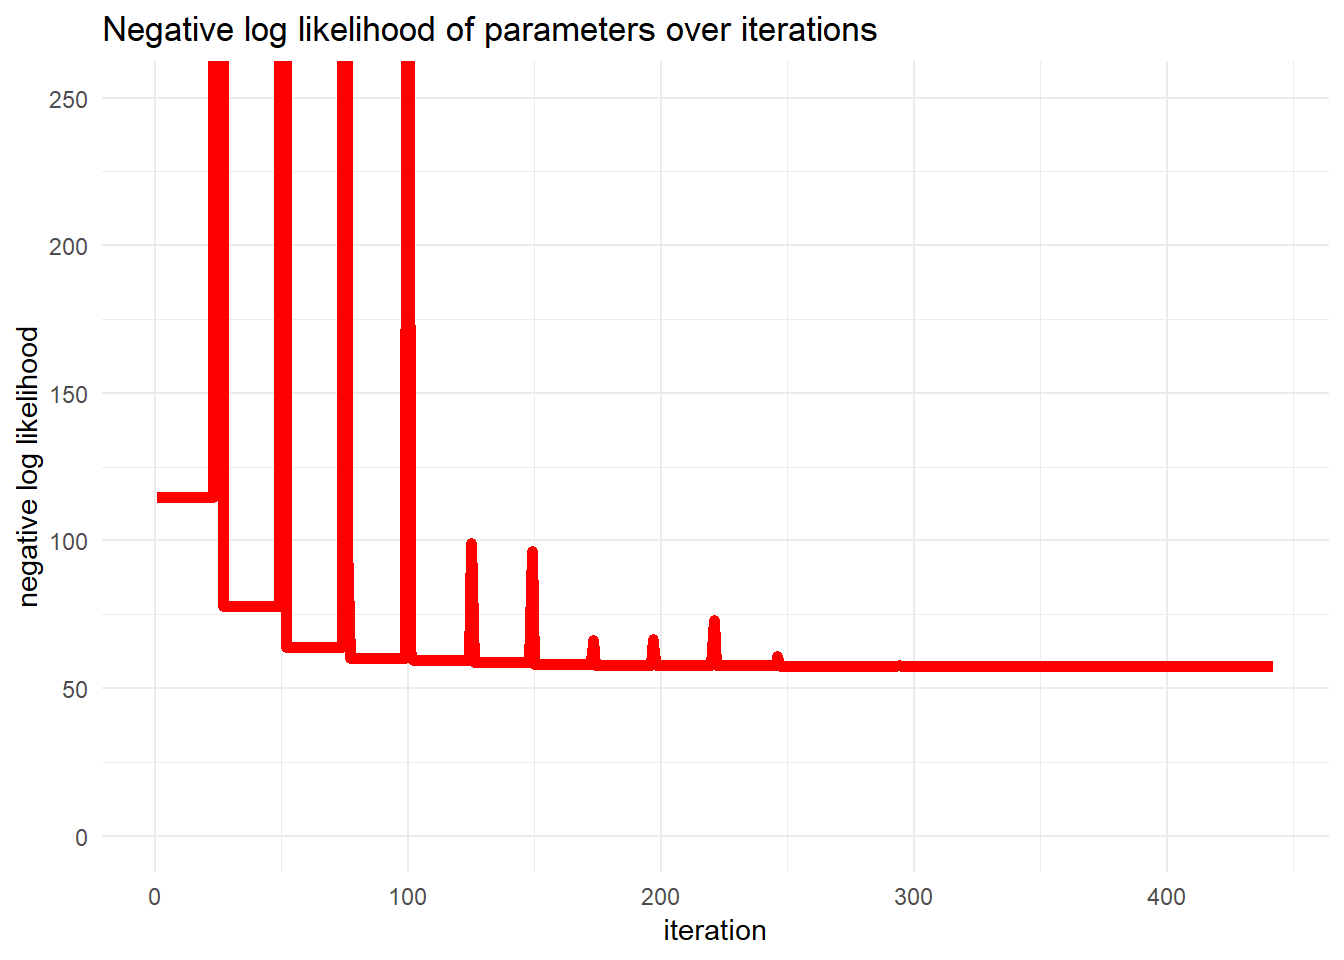
\includegraphics{2019-16-5-dixon-coles-1_files/figure-latex/plot_log_liks-1.pdf}

The final parameters can also be extracted from the output from optim()
and plotted:

\begin{Shaded}
\begin{Highlighting}[]
\NormalTok{p4 <-}\StringTok{ }\NormalTok{optimised_parameters4}\OperatorTok{$}\NormalTok{par }\OperatorTok
\StringTok{  }\CommentTok{# relist to add in first team}
\StringTok{  }\KeywordTok{relist_params}\NormalTok{() }\OperatorTok
\StringTok{  }\KeywordTok{unlist}\NormalTok{() }\OperatorTok
\StringTok{  }\CommentTok{# select team parameters}
\StringTok{  }\NormalTok{.[}\KeywordTok{grepl}\NormalTok{(}\StringTok{"beta|alpha"}\NormalTok{, }\KeywordTok{names}\NormalTok{(.))] }\OperatorTok
\StringTok{  }\KeywordTok{data.frame}\NormalTok{(}\DataTypeTok{value =}\NormalTok{ .,}
             \DataTypeTok{parameter =} \KeywordTok{names}\NormalTok{(.)) }\OperatorTok
\StringTok{  }\KeywordTok{separate}\NormalTok{(parameter, }\DataTypeTok{into =} \KeywordTok{c}\NormalTok{(}\StringTok{"parameter"}\NormalTok{, }\StringTok{"team"}\NormalTok{), }\StringTok{"}\CharTok{\textbackslash{}\textbackslash{}}\StringTok{."}\NormalTok{) }\OperatorTok
\StringTok{  }\CommentTok{# spread into wide format}
\StringTok{  }\KeywordTok{spread}\NormalTok{(parameter, value) }\OperatorTok
\StringTok{  }\CommentTok{# pipe into a plot}
\StringTok{  }\KeywordTok{ggplot}\NormalTok{(}\KeywordTok{aes}\NormalTok{(}\DataTypeTok{x =}\NormalTok{ alpha, }\DataTypeTok{y =}\NormalTok{ beta)) }\OperatorTok{+}
\StringTok{  }\KeywordTok{geom_point}\NormalTok{() }\OperatorTok{+}
\StringTok{  }\NormalTok{ggrepel}\OperatorTok{::}\KeywordTok{geom_text_repel}\NormalTok{(}\KeywordTok{aes}\NormalTok{(}\DataTypeTok{label =}\NormalTok{ team)) }\OperatorTok{+}
\StringTok{  }\KeywordTok{stat_smooth}\NormalTok{(}\DataTypeTok{method =} \StringTok{"lm"}\NormalTok{, }\DataTypeTok{se =} \OtherTok{FALSE}\NormalTok{) }\OperatorTok{+}
\StringTok{  }\KeywordTok{labs}\NormalTok{(}\DataTypeTok{title =} \StringTok{"Optimal parameters for teams"}\NormalTok{,}
       \DataTypeTok{subtitle =} \StringTok{"given first 8 weeks of results"}\NormalTok{,}
       \DataTypeTok{x =} \StringTok{"alpha (more likely to score ->)"}\NormalTok{,}
       \DataTypeTok{y =} \StringTok{"beta (less likely to concede ->)"}\NormalTok{) }\OperatorTok{+}
\StringTok{  }\KeywordTok{theme_minimal}\NormalTok{()}

\NormalTok{p4}
\end{Highlighting}
\end{Shaded}

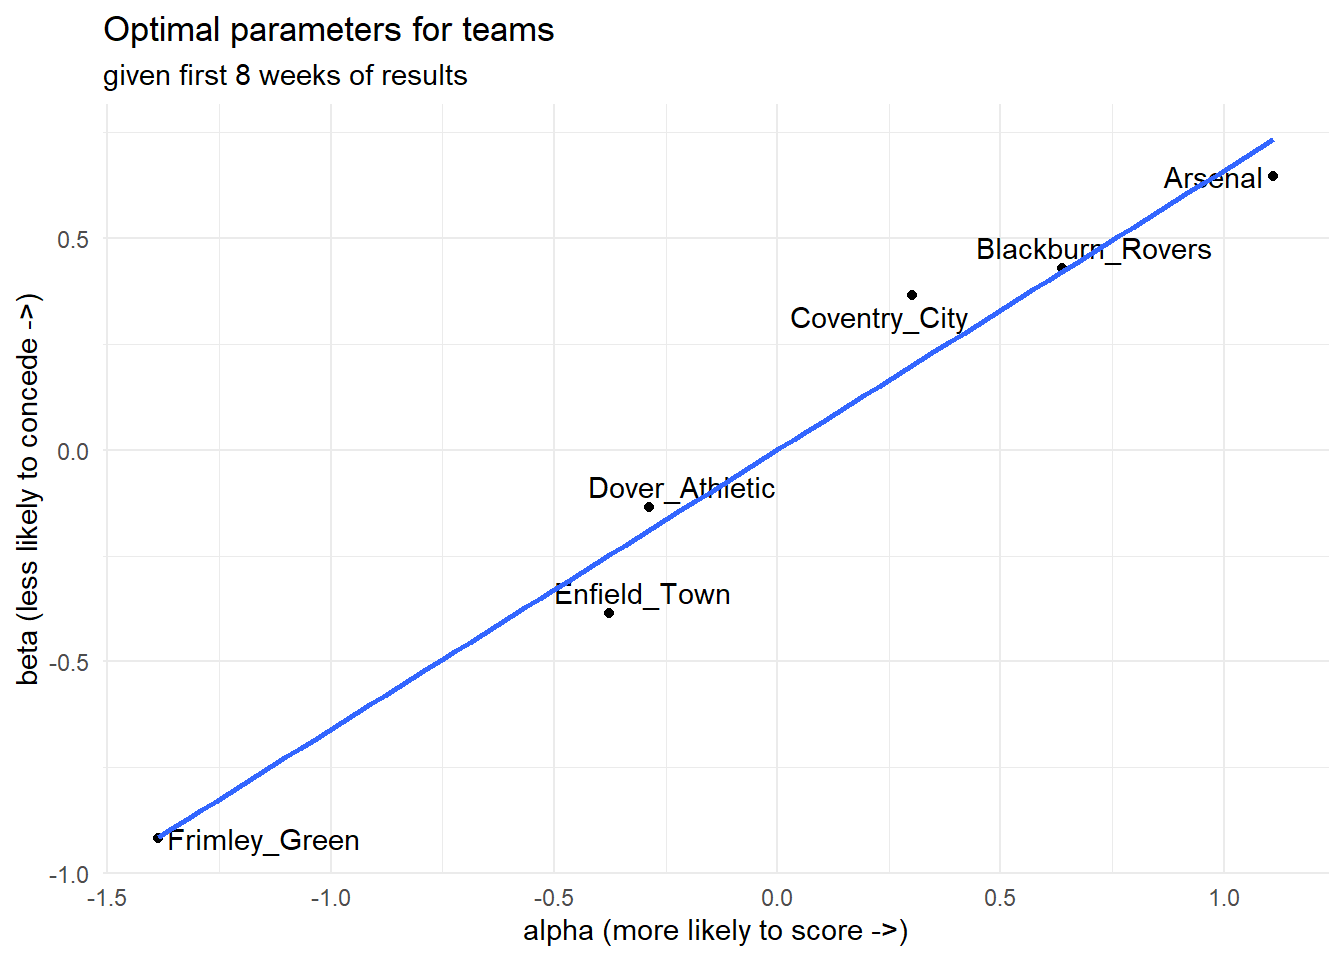
\includegraphics{2019-16-5-dixon-coles-1_files/figure-latex/plot_parameters-1.pdf}
Notice how the teams monotonically increase in both attack and defensive
ability. This is by design on how the results were created (see the
bottom of this post). With only 8 games per team however, there is quite
a lot of noise in the signal. Hitting the crossbar instead of scoring in
one game could make a fairly large difference in how the function rates
a team.

Also note how the regression line passes through the origin- this is a
result of us constraining the paramters to sum to zero.

\subsection{Predict Remaining Matches}\label{predict-remaining-matches}

Now we have rated each teams attack/defense, and the advantage to a team
to play at home, we can predict the remeaning matches between the teams.

For this, we just have to use the predict\_results() function we defined
earlier, except this time the output will be the expected goals per
team. Earlier we were measuring the deviance from expectation, but not
we assume the most likely result is exactly equal to the expected
results. If we wanted to we could work out how likely this result is,
and what the most likely results are.

This post is long enough however, so for now, we'll just detail the most
likely results.

\begin{Shaded}
\begin{Highlighting}[]
\NormalTok{predicted_results <-}\StringTok{ }\KeywordTok{predict_results}\NormalTok{(unplayed_games}\OperatorTok{$}\NormalTok{home,}
\NormalTok{                      unplayed_games}\OperatorTok{$}\NormalTok{away, }
                      \KeywordTok{relist_params}\NormalTok{(optimised_parameters4}\OperatorTok{$}\NormalTok{par)) }\OperatorTok
\StringTok{  }\KeywordTok{mutate_if}\NormalTok{(is.numeric, round, }\DecValTok{2}\NormalTok{) }\OperatorTok
\StringTok{  }\KeywordTok{print}\NormalTok{()}
\end{Highlighting}
\end{Shaded}

\begin{verbatim}
##               home             away e_hgoal e_agoal
## 1    Coventry_City          Arsenal    0.86    2.11
## 2 Blackburn_Rovers   Dover_Athletic    2.62    0.49
## 3    Frimley_Green     Enfield_Town    0.44    1.72
## 4          Arsenal Blackburn_Rovers    2.39    0.99
## 5    Coventry_City    Frimley_Green    4.09    0.17
## 6   Dover_Athletic     Enfield_Town    1.33    0.79
\end{verbatim}

All of these look reasonable, with better teams beaten worse ones. The
only match that the model thinks might well end in a draw is Dover at
home to Enfield, which is not entirely unreasonable.

We can add these predictions to our earlier matrix of results to get a
sense if these fit in with the trend from the observed matches:

\begin{Shaded}
\begin{Highlighting}[]
\NormalTok{p5 <-}\StringTok{ }\KeywordTok{rbind}\NormalTok{(}
\NormalTok{  predicted_results }\OperatorTok
\StringTok{    }\KeywordTok{rename_if}\NormalTok{(is.numeric, gsub, }\DataTypeTok{pattern =} \StringTok{"e_"}\NormalTok{, }\DataTypeTok{replacement =} \StringTok{""}\NormalTok{) }\OperatorTok
\StringTok{    }\KeywordTok{mutate}\NormalTok{(}\DataTypeTok{type =} \StringTok{"predicted"}\NormalTok{),}
\NormalTok{  results }\OperatorTok
\StringTok{    }\KeywordTok{select}\NormalTok{(}\OperatorTok{-}\NormalTok{gameweek) }\OperatorTok
\StringTok{    }\KeywordTok{mutate}\NormalTok{(}\DataTypeTok{type =} \StringTok{"result"}\NormalTok{)}
\NormalTok{) }\OperatorTok
\StringTok{  }\KeywordTok{ggplot}\NormalTok{(., }\KeywordTok{aes}\NormalTok{(}\DataTypeTok{x =}\NormalTok{ away, }\DataTypeTok{y =}\NormalTok{ home, }\DataTypeTok{fill =}\NormalTok{ hgoal}\OperatorTok{-}\NormalTok{agoal)) }\OperatorTok{+}
\StringTok{  }\KeywordTok{geom_tile}\NormalTok{() }\OperatorTok{+}
\StringTok{  }\CommentTok{# add the scorelines}
\StringTok{  }\KeywordTok{geom_label}\NormalTok{(}\KeywordTok{aes}\NormalTok{(}\DataTypeTok{label =} \KeywordTok{paste}\NormalTok{(hgoal, agoal, }\DataTypeTok{sep =} \StringTok{"-"}\NormalTok{), }\DataTypeTok{colour =}\NormalTok{ type), }\DataTypeTok{fill =} \StringTok{"white"}\NormalTok{) }\OperatorTok{+}
\StringTok{  }\CommentTok{# colour where black for actual results and red for predictions}
\StringTok{  }\KeywordTok{scale_colour_manual}\NormalTok{(}\DataTypeTok{values =} \KeywordTok{c}\NormalTok{(}\StringTok{"red"}\NormalTok{, }\StringTok{"black"}\NormalTok{)) }\OperatorTok{+}
\StringTok{  }\CommentTok{# colour where green shows home win and red an away win}
\StringTok{  }\KeywordTok{scale_fill_gradient2}\NormalTok{(}\DataTypeTok{low =} \StringTok{"darkred"}\NormalTok{, }\DataTypeTok{high =} \StringTok{"green"}\NormalTok{, }\DataTypeTok{midpoint =} \DecValTok{0}\NormalTok{, }\DataTypeTok{guide =} \OtherTok{FALSE}\NormalTok{) }\OperatorTok{+}
\StringTok{  }\KeywordTok{scale_x_discrete}\NormalTok{(}\DataTypeTok{limits =} \KeywordTok{levels}\NormalTok{(results}\OperatorTok{$}\NormalTok{home), }\DataTypeTok{position =} \StringTok{"top"}\NormalTok{) }\OperatorTok{+}
\StringTok{  }\KeywordTok{scale_y_discrete}\NormalTok{(}\DataTypeTok{limits =} \KeywordTok{rev}\NormalTok{(}\KeywordTok{levels}\NormalTok{(results}\OperatorTok{$}\NormalTok{away))) }\OperatorTok{+}
\StringTok{  }\KeywordTok{theme_minimal}\NormalTok{()}

\NormalTok{p5}
\end{Highlighting}
\end{Shaded}

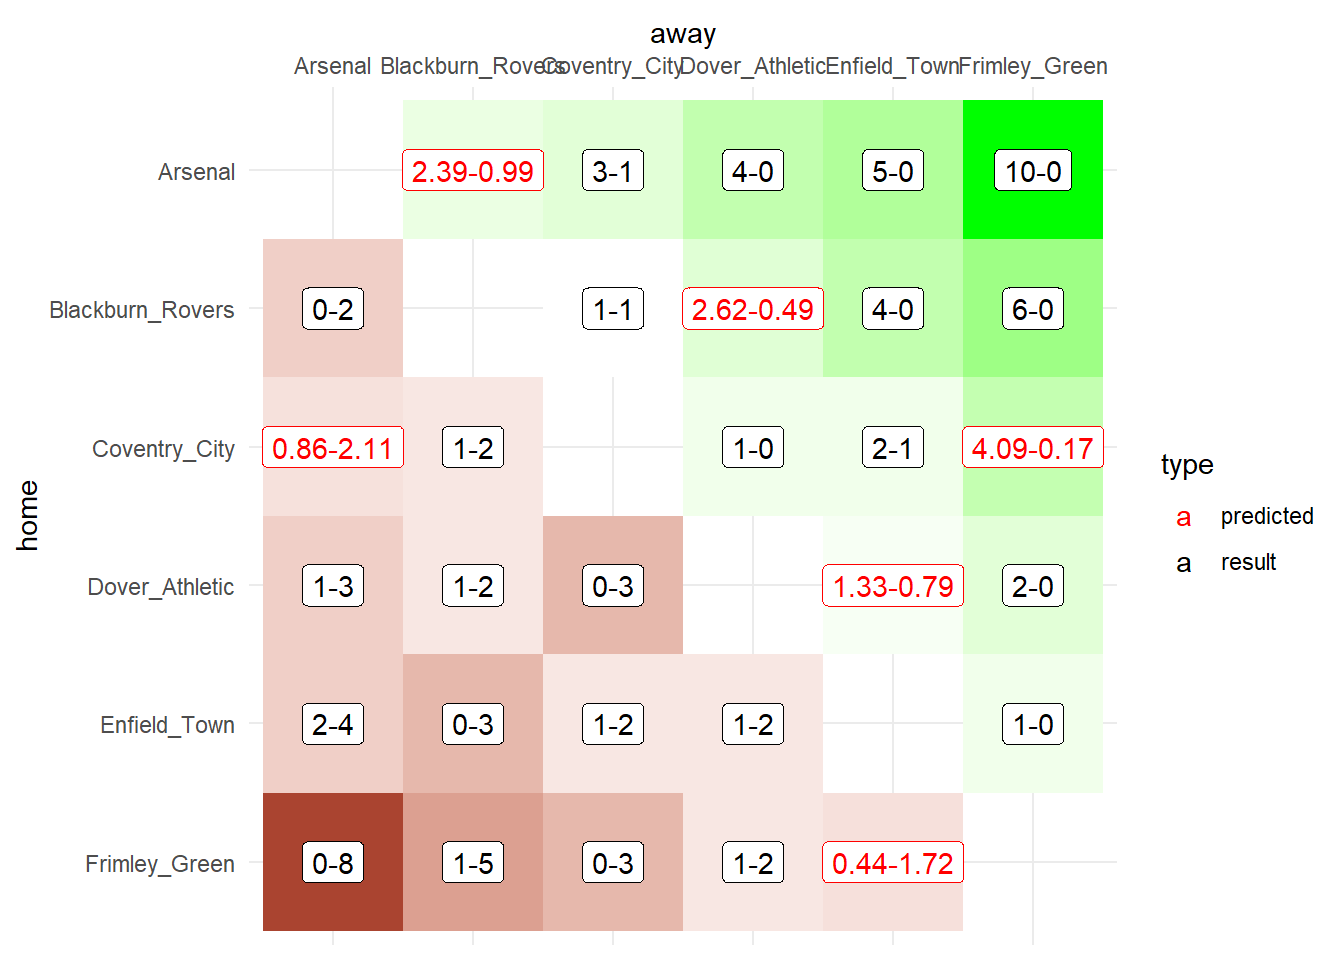
\includegraphics{2019-16-5-dixon-coles-1_files/figure-latex/plot_all_games-1.pdf}

Which they do! The predicted results fit in with the gradient of heavier
defeats for home teams towards the bottom left, progressing to easy home
victories in the top right.

That's all for this post. Hopefully using the Poisson distributon to
model football matches is a little clearer now. Feel free to email me
any questions and check out the packages I stole all the codes/idea
from.

Next time, I'll go over how to predict how likely a range of results are
for any single match in (hopefully) a shorter post; until then!

1 much of the code I use here is stolen/reworked from the code shared on
this repo

2 towards the end of writing this post I came across
\href{https://dashee87.github.io/football/python/predicting-football-results-with-statistical-modelling-dixon-coles-and-time-weighting/}{David
Sheehan's blog} which actually does a pretty good job, but I felt still
didn't quite go through how/why the model uses the maths it does

3 see \url{https://arxiv.org/pdf/cond-mat/0110605.pdf} and also the
conclusion of
\href{https://dashee87.github.io/football/python/predicting-football-results-with-statistical-modelling/}{David
Sheehan's blog on Dixon-Coles processes}

4 *we could instead \emph{maximise} the sum of the log likelihoods and
then the error will converge towards 0 from a negative number. Either is
fine.

\subsection{Results generation}\label{results-generation}

First we need to create a df of fixtures for each team

\begin{Shaded}
\begin{Highlighting}[]
\CommentTok{# https://stackoverflow.com/questions/54099990/is-there-an-efficient-algorithm-to-create-this-type-of-schedule}
\NormalTok{create_fixtures <-}\StringTok{ }\ControlFlowTok{function}\NormalTok{(teams) \{}
  \CommentTok{# keep team 1 in place}
\NormalTok{  team1 <-}\StringTok{ }\KeywordTok{as.character}\NormalTok{(teams[}\DecValTok{1}\NormalTok{])}
  \CommentTok{#rotate other teams around team 1}
\NormalTok{  other_teams <-}\StringTok{ }\KeywordTok{as.character}\NormalTok{(teams[}\OperatorTok{!}\NormalTok{teams }\OperatorTok\StringTok{ }\NormalTok{team1])}
\NormalTok{  length <-}\StringTok{ }\KeywordTok{length}\NormalTok{(other_teams)}
  
  \CommentTok{# generate fixtures each week}
  \ControlFlowTok{for}\NormalTok{(week }\ControlFlowTok{in} \KeywordTok{seq}\NormalTok{((}\KeywordTok{length}\NormalTok{(teams)}\OperatorTok{-}\DecValTok{1}\NormalTok{)}\OperatorTok{*}\DecValTok{2}\NormalTok{)) \{}
    
    \ControlFlowTok{if}\NormalTok{(week }\OperatorTok\StringTok{ }\DecValTok{2} \OperatorTok{==}\StringTok{ }\DecValTok{0}\NormalTok{) \{}
\NormalTok{      fixtures <-}\StringTok{ }\KeywordTok{data.frame}\NormalTok{(}\DataTypeTok{home =} \KeywordTok{c}\NormalTok{(team1, other_teams[}\DecValTok{1}\OperatorTok{:}\DecValTok{2}\NormalTok{]),}
                             \DataTypeTok{away =}\NormalTok{ other_teams[length}\OperatorTok{:}\DecValTok{3}\NormalTok{],}
                             \DataTypeTok{gameweek =}\NormalTok{ week)}
\NormalTok{    \} }\ControlFlowTok{else}\NormalTok{ \{}
\NormalTok{      fixtures <-}\StringTok{ }\KeywordTok{data.frame}\NormalTok{(}\DataTypeTok{home =}\NormalTok{ other_teams[length}\OperatorTok{:}\DecValTok{3}\NormalTok{],}
                             \DataTypeTok{away =} \KeywordTok{c}\NormalTok{(team1, other_teams[}\DecValTok{1}\OperatorTok{:}\DecValTok{2}\NormalTok{]),}
                             \DataTypeTok{gameweek =}\NormalTok{ week)}
      
\NormalTok{    \}}
    
    \ControlFlowTok{if}\NormalTok{(week }\OperatorTok{==}\StringTok{ }\DecValTok{1}\NormalTok{) \{}
\NormalTok{      fixtures_df <-}\StringTok{ }\NormalTok{fixtures }
\NormalTok{    \} }\ControlFlowTok{else}\NormalTok{ \{}
\NormalTok{      fixtures_df <-}\StringTok{ }\KeywordTok{rbind}\NormalTok{(fixtures_df, fixtures)}
\NormalTok{    \}}
    
    \CommentTok{# rotate other teams around}
\NormalTok{    other_teams <-}\StringTok{ }\KeywordTok{c}\NormalTok{(other_teams[length], other_teams[}\DecValTok{1}\OperatorTok{:}\NormalTok{length}\OperatorTok{-}\DecValTok{1}\NormalTok{])}
\NormalTok{  \}}
  
  \KeywordTok{return}\NormalTok{(fixtures_df)}
\NormalTok{\}}

\CommentTok{# create the fixtures}
\NormalTok{fixtures <-}\StringTok{ }\KeywordTok{create_fixtures}\NormalTok{(teams) }\OperatorTok
\StringTok{  }\KeywordTok{mutate_if}\NormalTok{(is.factor, as.character)}

\CommentTok{# print the fixture list}
\NormalTok{fixtures}
\end{Highlighting}
\end{Shaded}

\begin{verbatim}
##                home             away gameweek
## 1     Frimley_Green          Arsenal        1
## 2      Enfield_Town Blackburn_Rovers        1
## 3    Dover_Athletic    Coventry_City        1
## 4           Arsenal     Enfield_Town        2
## 5     Frimley_Green   Dover_Athletic        2
## 6  Blackburn_Rovers    Coventry_City        2
## 7    Dover_Athletic          Arsenal        3
## 8     Coventry_City     Enfield_Town        3
## 9  Blackburn_Rovers    Frimley_Green        3
## 10          Arsenal    Coventry_City        4
## 11   Dover_Athletic Blackburn_Rovers        4
## 12     Enfield_Town    Frimley_Green        4
## 13 Blackburn_Rovers          Arsenal        5
## 14    Frimley_Green    Coventry_City        5
## 15     Enfield_Town   Dover_Athletic        5
## 16          Arsenal    Frimley_Green        6
## 17 Blackburn_Rovers     Enfield_Town        6
## 18    Coventry_City   Dover_Athletic        6
## 19     Enfield_Town          Arsenal        7
## 20   Dover_Athletic    Frimley_Green        7
## 21    Coventry_City Blackburn_Rovers        7
## 22          Arsenal   Dover_Athletic        8
## 23     Enfield_Town    Coventry_City        8
## 24    Frimley_Green Blackburn_Rovers        8
## 25    Coventry_City          Arsenal        9
## 26 Blackburn_Rovers   Dover_Athletic        9
## 27    Frimley_Green     Enfield_Town        9
## 28          Arsenal Blackburn_Rovers       10
## 29    Coventry_City    Frimley_Green       10
## 30   Dover_Athletic     Enfield_Town       10
\end{verbatim}

and then create the results

\begin{Shaded}
\begin{Highlighting}[]
\CommentTok{# using goalmodel package }
\CommentTok{# https://github.com/opisthokonta/goalmodel}
\KeywordTok{library}\NormalTok{(goalmodel)}

\CommentTok{# have to manually create a list of parameters}
\NormalTok{model <-}\StringTok{ }\KeywordTok{list}\NormalTok{()}
\CommentTok{# stratify teams abilities in attack and defense}
\NormalTok{model}\OperatorTok{$}\NormalTok{parameters <-}\StringTok{ }\KeywordTok{list}\NormalTok{(}\DataTypeTok{attack =} \KeywordTok{seq}\NormalTok{(}\DecValTok{1}\NormalTok{, }\OperatorTok{-}\DecValTok{1} \OperatorTok{+}\StringTok{ }\DecValTok{2}\OperatorTok{/}\KeywordTok{length}\NormalTok{(teams), }\DataTypeTok{by =} \OperatorTok{-}\DecValTok{2}\OperatorTok{/}\NormalTok{(}\KeywordTok{length}\NormalTok{(teams)}\OperatorTok{-}\DecValTok{1}\NormalTok{)) }\OperatorTok
\StringTok{                           }\KeywordTok{append}\NormalTok{(}\OperatorTok{-}\KeywordTok{sum}\NormalTok{(.)) }\OperatorTok
\StringTok{                           `}\DataTypeTok{names<-}\StringTok{`}\NormalTok{(teams), }
                         \DataTypeTok{defense =} \KeywordTok{seq}\NormalTok{(}\DecValTok{1}\NormalTok{, }\OperatorTok{-}\DecValTok{1} \OperatorTok{+}\StringTok{ }\DecValTok{2}\OperatorTok{/}\KeywordTok{length}\NormalTok{(teams), }\DataTypeTok{by =} \OperatorTok{-}\DecValTok{2}\OperatorTok{/}\NormalTok{(}\KeywordTok{length}\NormalTok{(teams)}\OperatorTok{-}\DecValTok{1}\NormalTok{)) }\OperatorTok
\StringTok{                           }\KeywordTok{append}\NormalTok{(}\OperatorTok{-}\KeywordTok{sum}\NormalTok{(.)) }\OperatorTok
\StringTok{                           `}\DataTypeTok{names<-}\StringTok{`}\NormalTok{(teams), }
                         \CommentTok{# no base rate of goals}
                         \DataTypeTok{intercept =} \DecValTok{0}\NormalTok{, }
                         \CommentTok{# roughly accurate hfa for English professional football}
                         \DataTypeTok{hfa =} \FloatTok{0.3}\NormalTok{)}

\CommentTok{# add in teams}
\NormalTok{model}\OperatorTok{$}\NormalTok{all_teams <-}\StringTok{ }\NormalTok{teams}
\CommentTok{# use a simple Poisson model with 8 goals max}
\NormalTok{model}\OperatorTok{$}\NormalTok{model <-}\StringTok{ "poisson"}
\NormalTok{model}\OperatorTok{$}\NormalTok{maxgoal <-}\StringTok{ }\DecValTok{8}

\CommentTok{# use the model to predict results using regista package}
\NormalTok{results <-}\StringTok{ }\KeywordTok{predict_expg}\NormalTok{(model, fixtures}\OperatorTok{$}\NormalTok{home, fixtures}\OperatorTok{$}\NormalTok{away, }\DataTypeTok{return_df =} \OtherTok{TRUE}\NormalTok{) }\OperatorTok
\StringTok{  }\CommentTok{# add some noise}
\StringTok{  }\KeywordTok{mutate}\NormalTok{(}\DataTypeTok{noise1 =} \KeywordTok{rnorm}\NormalTok{(}\KeywordTok{nrow}\NormalTok{(.), }\DecValTok{0}\NormalTok{, }\FloatTok{0.5}\NormalTok{),}
         \DataTypeTok{noise2 =} \KeywordTok{rnorm}\NormalTok{(}\KeywordTok{nrow}\NormalTok{(.), }\DecValTok{0}\NormalTok{, }\FloatTok{0.5}\NormalTok{)) }\OperatorTok
\StringTok{  }\KeywordTok{mutate}\NormalTok{(}\DataTypeTok{hgoal =} \KeywordTok{round}\NormalTok{(expg1 }\OperatorTok{+}\StringTok{ }\NormalTok{noise1,}\DecValTok{0}\NormalTok{ ),}
         \DataTypeTok{agoal =} \KeywordTok{round}\NormalTok{(expg2 }\OperatorTok{+}\StringTok{ }\NormalTok{noise2,}\DecValTok{0}\NormalTok{),}
         \DataTypeTok{home =} \KeywordTok{as.factor}\NormalTok{(team1),}
         \DataTypeTok{away =} \KeywordTok{as.factor}\NormalTok{(team2)) }\OperatorTok
\StringTok{  }\CommentTok{# merge to fixtures}
\StringTok{  }\KeywordTok{merge}\NormalTok{(., fixtures, }\DataTypeTok{by =} \KeywordTok{c}\NormalTok{(}\StringTok{"home"}\NormalTok{, }\StringTok{"away"}\NormalTok{)) }\OperatorTok
\StringTok{  }\CommentTok{# cant score less than zero goals}
\StringTok{  }\KeywordTok{mutate_at}\NormalTok{(}\KeywordTok{vars}\NormalTok{(hgoal}\OperatorTok{:}\NormalTok{agoal), }\KeywordTok{funs}\NormalTok{(}\KeywordTok{replace}\NormalTok{(., .}\OperatorTok{<}\DecValTok{0}\NormalTok{, }\DecValTok{0}\NormalTok{))) }\OperatorTok
\StringTok{  }\KeywordTok{select}\NormalTok{(home, away, hgoal, agoal, gameweek) }\OperatorTok
\StringTok{  }\KeywordTok{arrange}\NormalTok{(gameweek, home) }\OperatorTok
\StringTok{  }\CommentTok{# treat only first 8 weeks as played}
\StringTok{  }\KeywordTok{filter}\NormalTok{(gameweek }\OperatorTok{<=}\StringTok{ }\DecValTok{8}\NormalTok{)}

\CommentTok{# print results}
\NormalTok{results}
\end{Highlighting}
\end{Shaded}

\begin{verbatim}
##                home             away hgoal agoal gameweek
## 1    Dover_Athletic    Coventry_City     2     3        1
## 2      Enfield_Town Blackburn_Rovers     0     3        1
## 3     Frimley_Green          Arsenal     0     8        1
## 4           Arsenal     Enfield_Town     7     0        2
## 5  Blackburn_Rovers    Coventry_City     2     1        2
## 6     Frimley_Green   Dover_Athletic     1     3        2
## 7  Blackburn_Rovers    Frimley_Green     6     1        3
## 8     Coventry_City     Enfield_Town     3     0        3
## 9    Dover_Athletic          Arsenal     0     3        3
## 10          Arsenal    Coventry_City     3     0        4
## 11   Dover_Athletic Blackburn_Rovers     0     3        4
## 12     Enfield_Town    Frimley_Green     1     0        4
## 13 Blackburn_Rovers          Arsenal     1     1        5
## 14     Enfield_Town   Dover_Athletic     1     1        5
## 15    Frimley_Green    Coventry_City     1     4        5
## 16          Arsenal    Frimley_Green    10     1        6
## 17 Blackburn_Rovers     Enfield_Town     5     0        6
## 18    Coventry_City   Dover_Athletic     2     0        6
## 19    Coventry_City Blackburn_Rovers     1     2        7
## 20   Dover_Athletic    Frimley_Green     3     1        7
## 21     Enfield_Town          Arsenal     0     5        7
## 22          Arsenal   Dover_Athletic     4     1        8
## 23     Enfield_Town    Coventry_City     1     2        8
## 24    Frimley_Green Blackburn_Rovers     0     4        8
\end{verbatim}


\end{document}
